\section{系统实现}

\subsection{系统管理员端}

\subsubsection{参数设置:}
在参数设置模块中,管理员可以对专业、教师提交题目截止时间、管理员审核题目截止时间、
学生第一次选题开始时间、学生第一次选题截止时间、管理员第一次匹配截止时间
学生第二次选题截止时间、管理员第二次匹配截止时间进行设置。
\begin{figure}[ht] % "h" 表示图片放置在文本所在位置,也可以使用其他选项
    \centering
    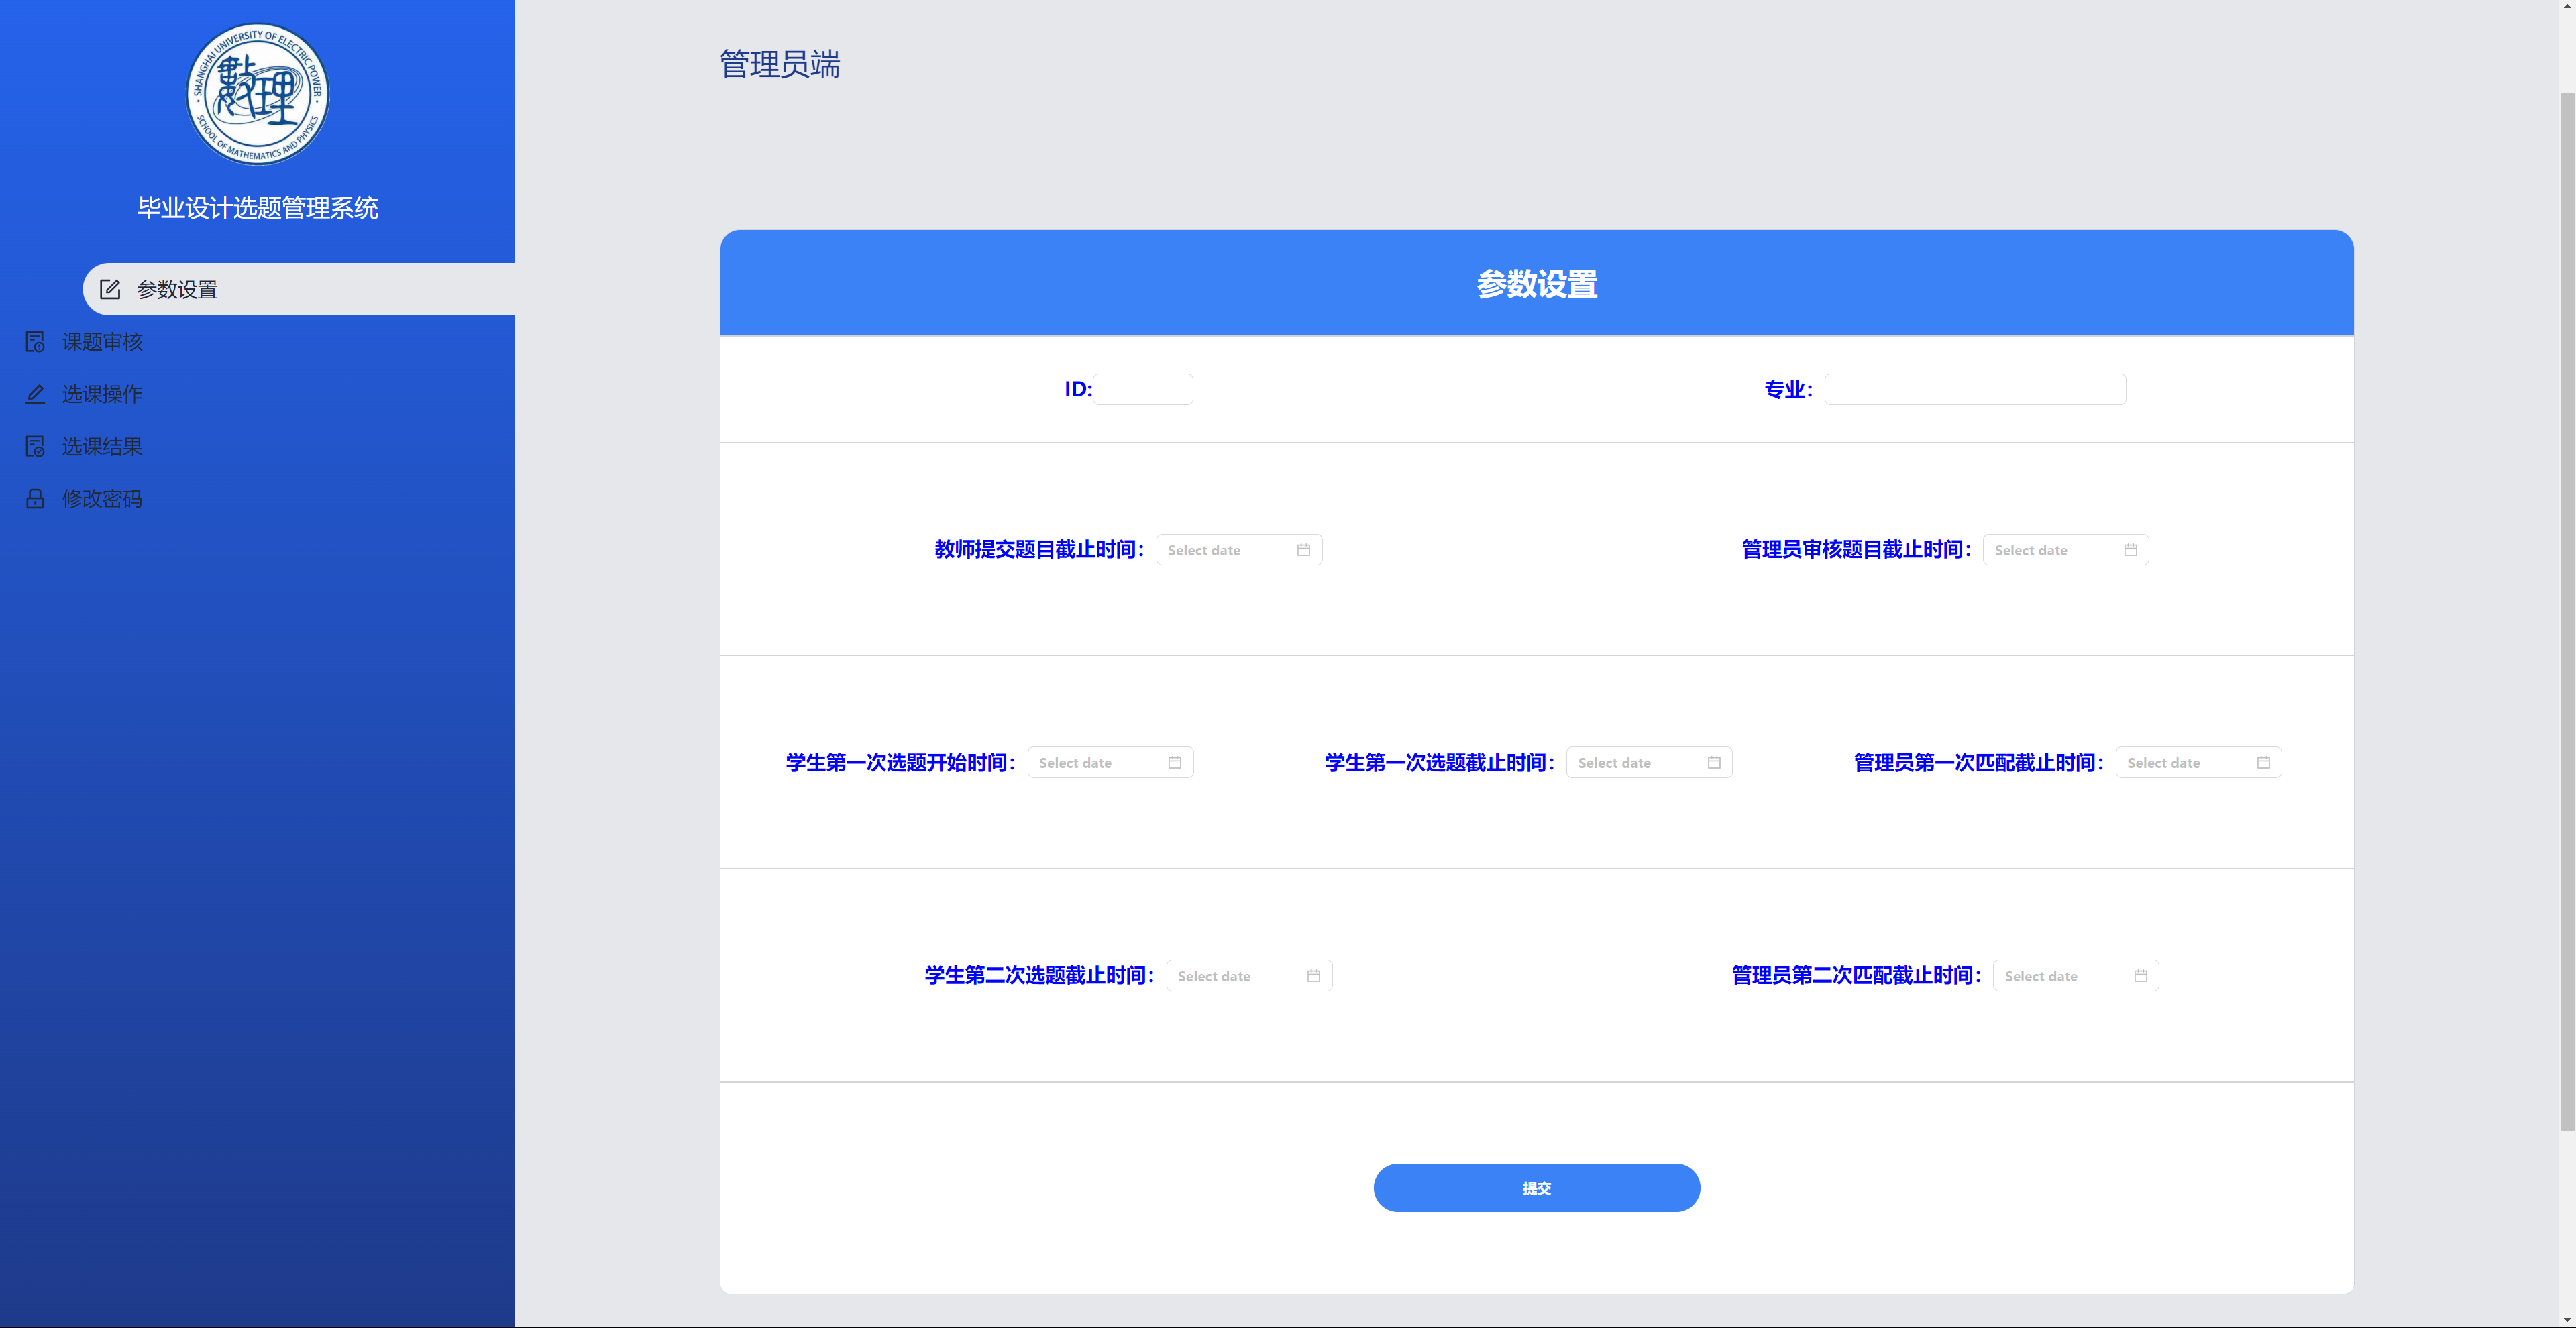
\includegraphics[width=1\textwidth]{管理员端01.png} % 插入图片并指定宽度
    \caption{管理员端-参数设置} % 添加图片标题
    \label{fig:manager01} % 为图片添加标签,以便在文本中引用
\end{figure}

\clearpage

\subsubsection{课题审核:}
在课题审核模块中,系统管理员可以查看到课题的编号、名称、指导老师、所属专业年级以及审核情况,
并对课题进行审核操作。
\begin{figure}[h]
    \centering
    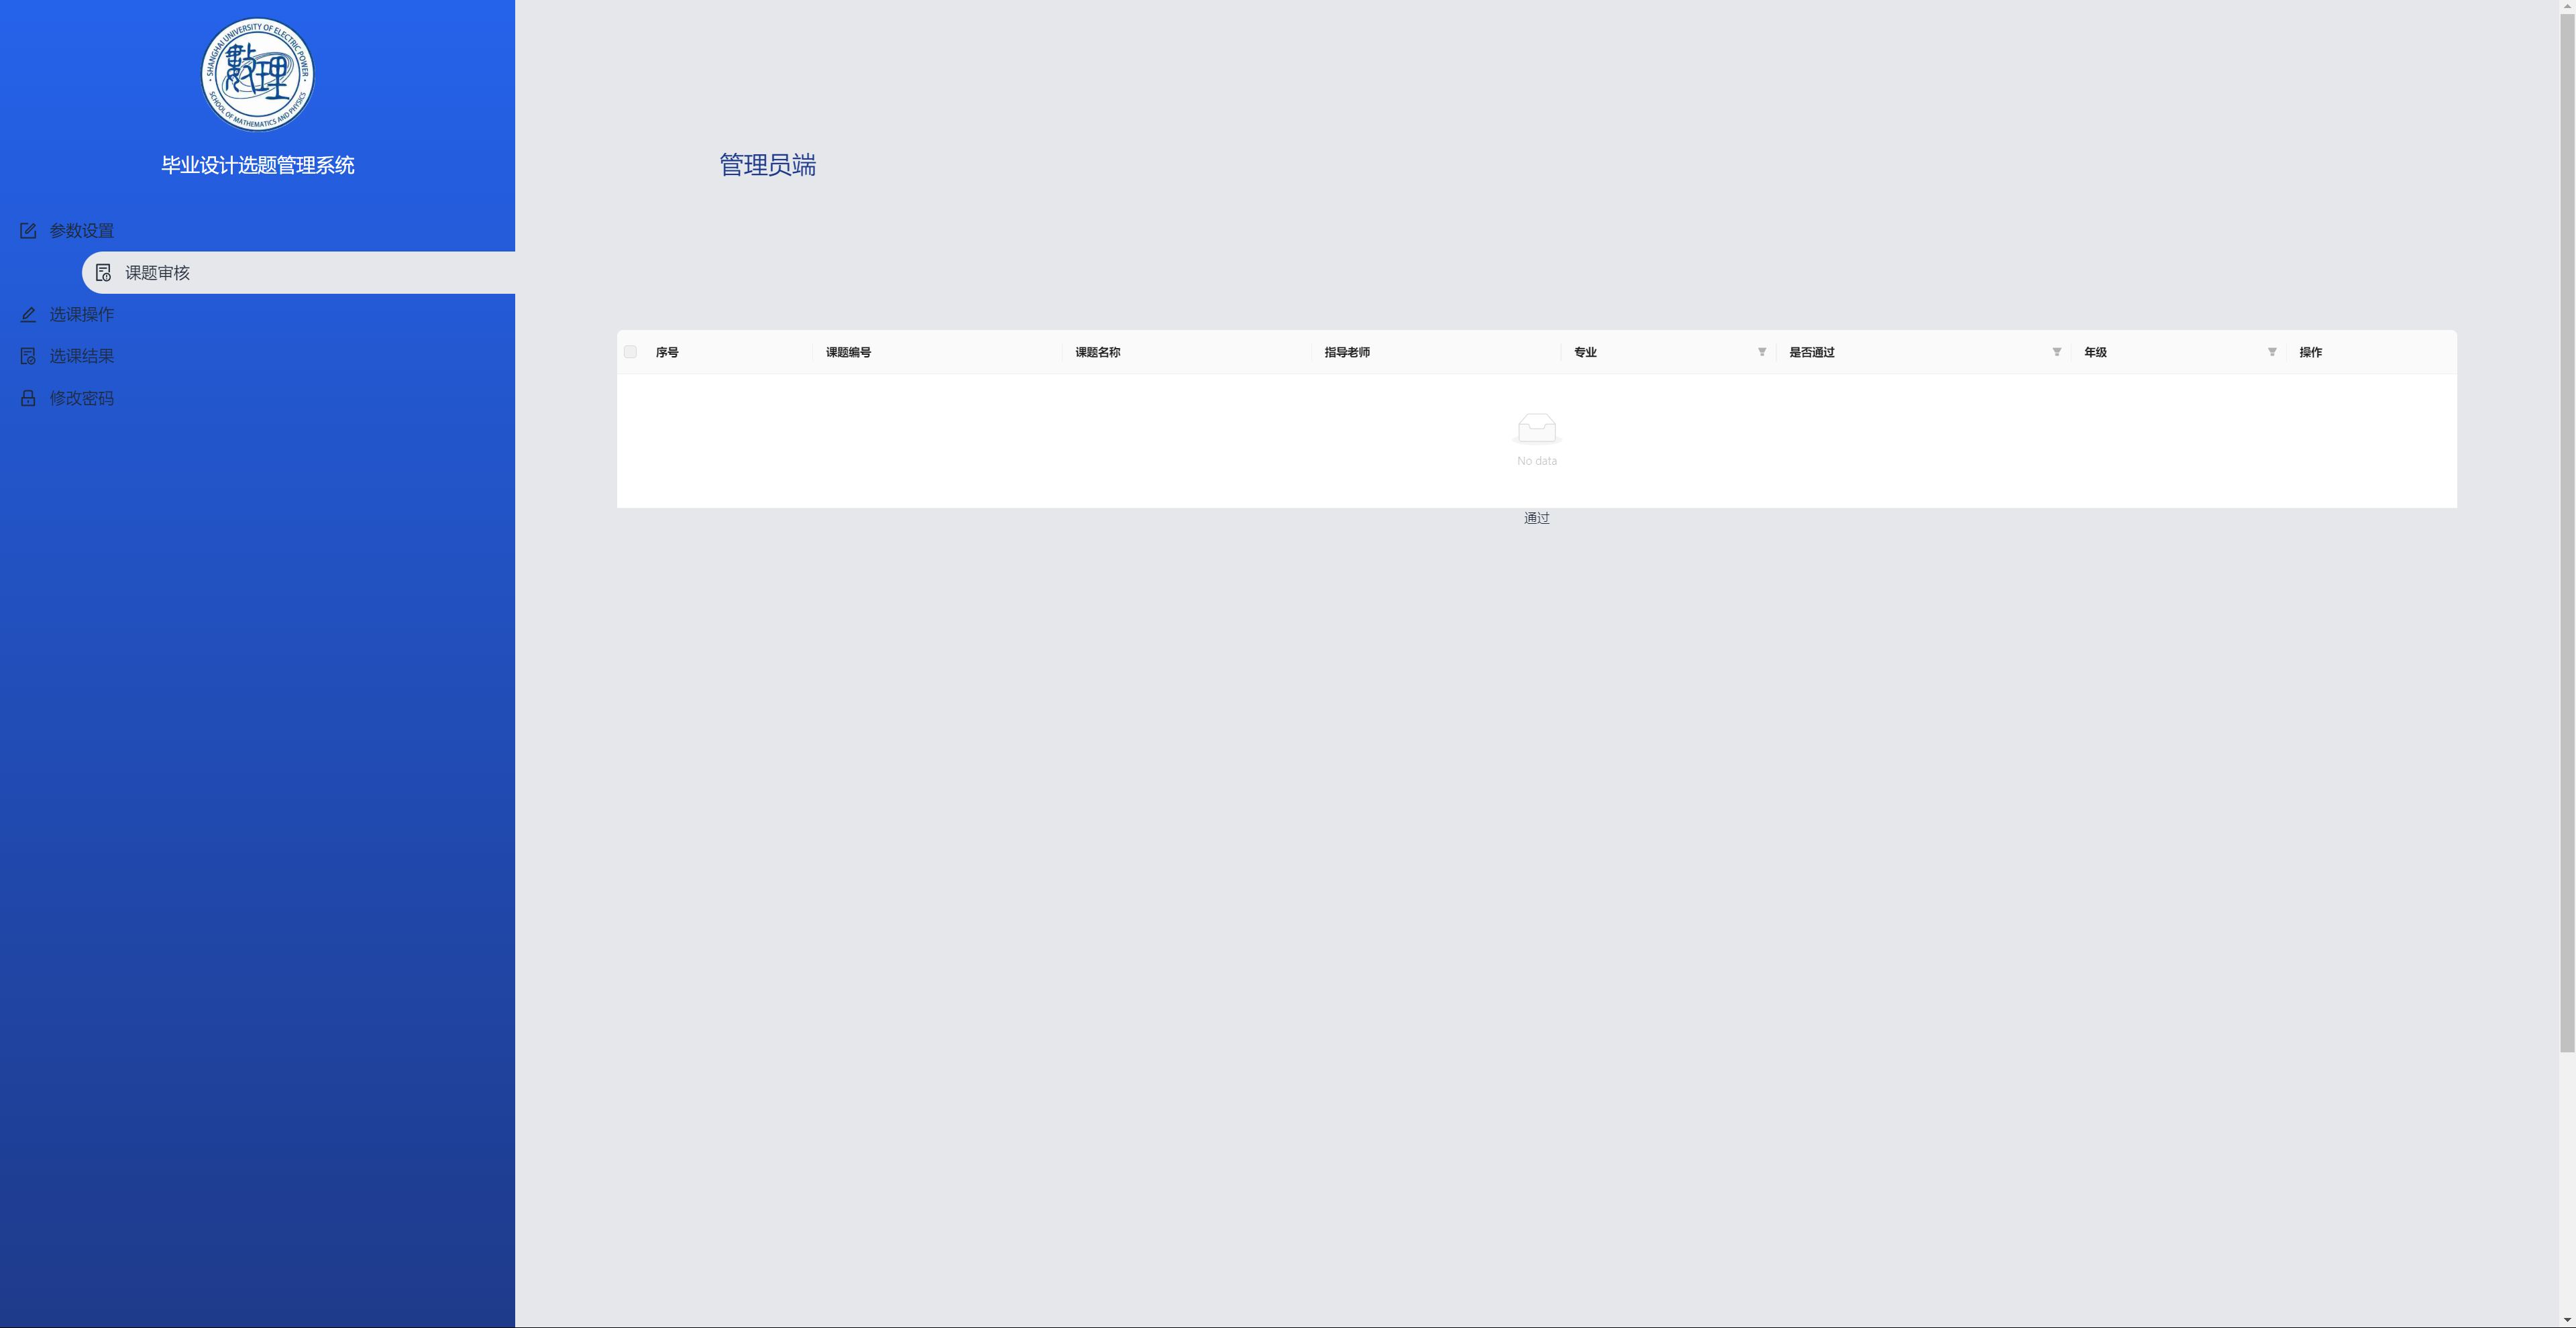
\includegraphics[width=1\textwidth]{images/管理员端02.png}
    \caption{管理员端-课题审核}
    \label{fig:manager02}
\end{figure}

\subsubsection{选课操作:}
在选课操作界面,系统管理员可以设置提前批选课的学号以及课号,
查看第一第二次选题分配情况,并且提供了导出选题匹配结果以及选题失败同学名单的选项。
\begin{figure}[h]
    \centering
    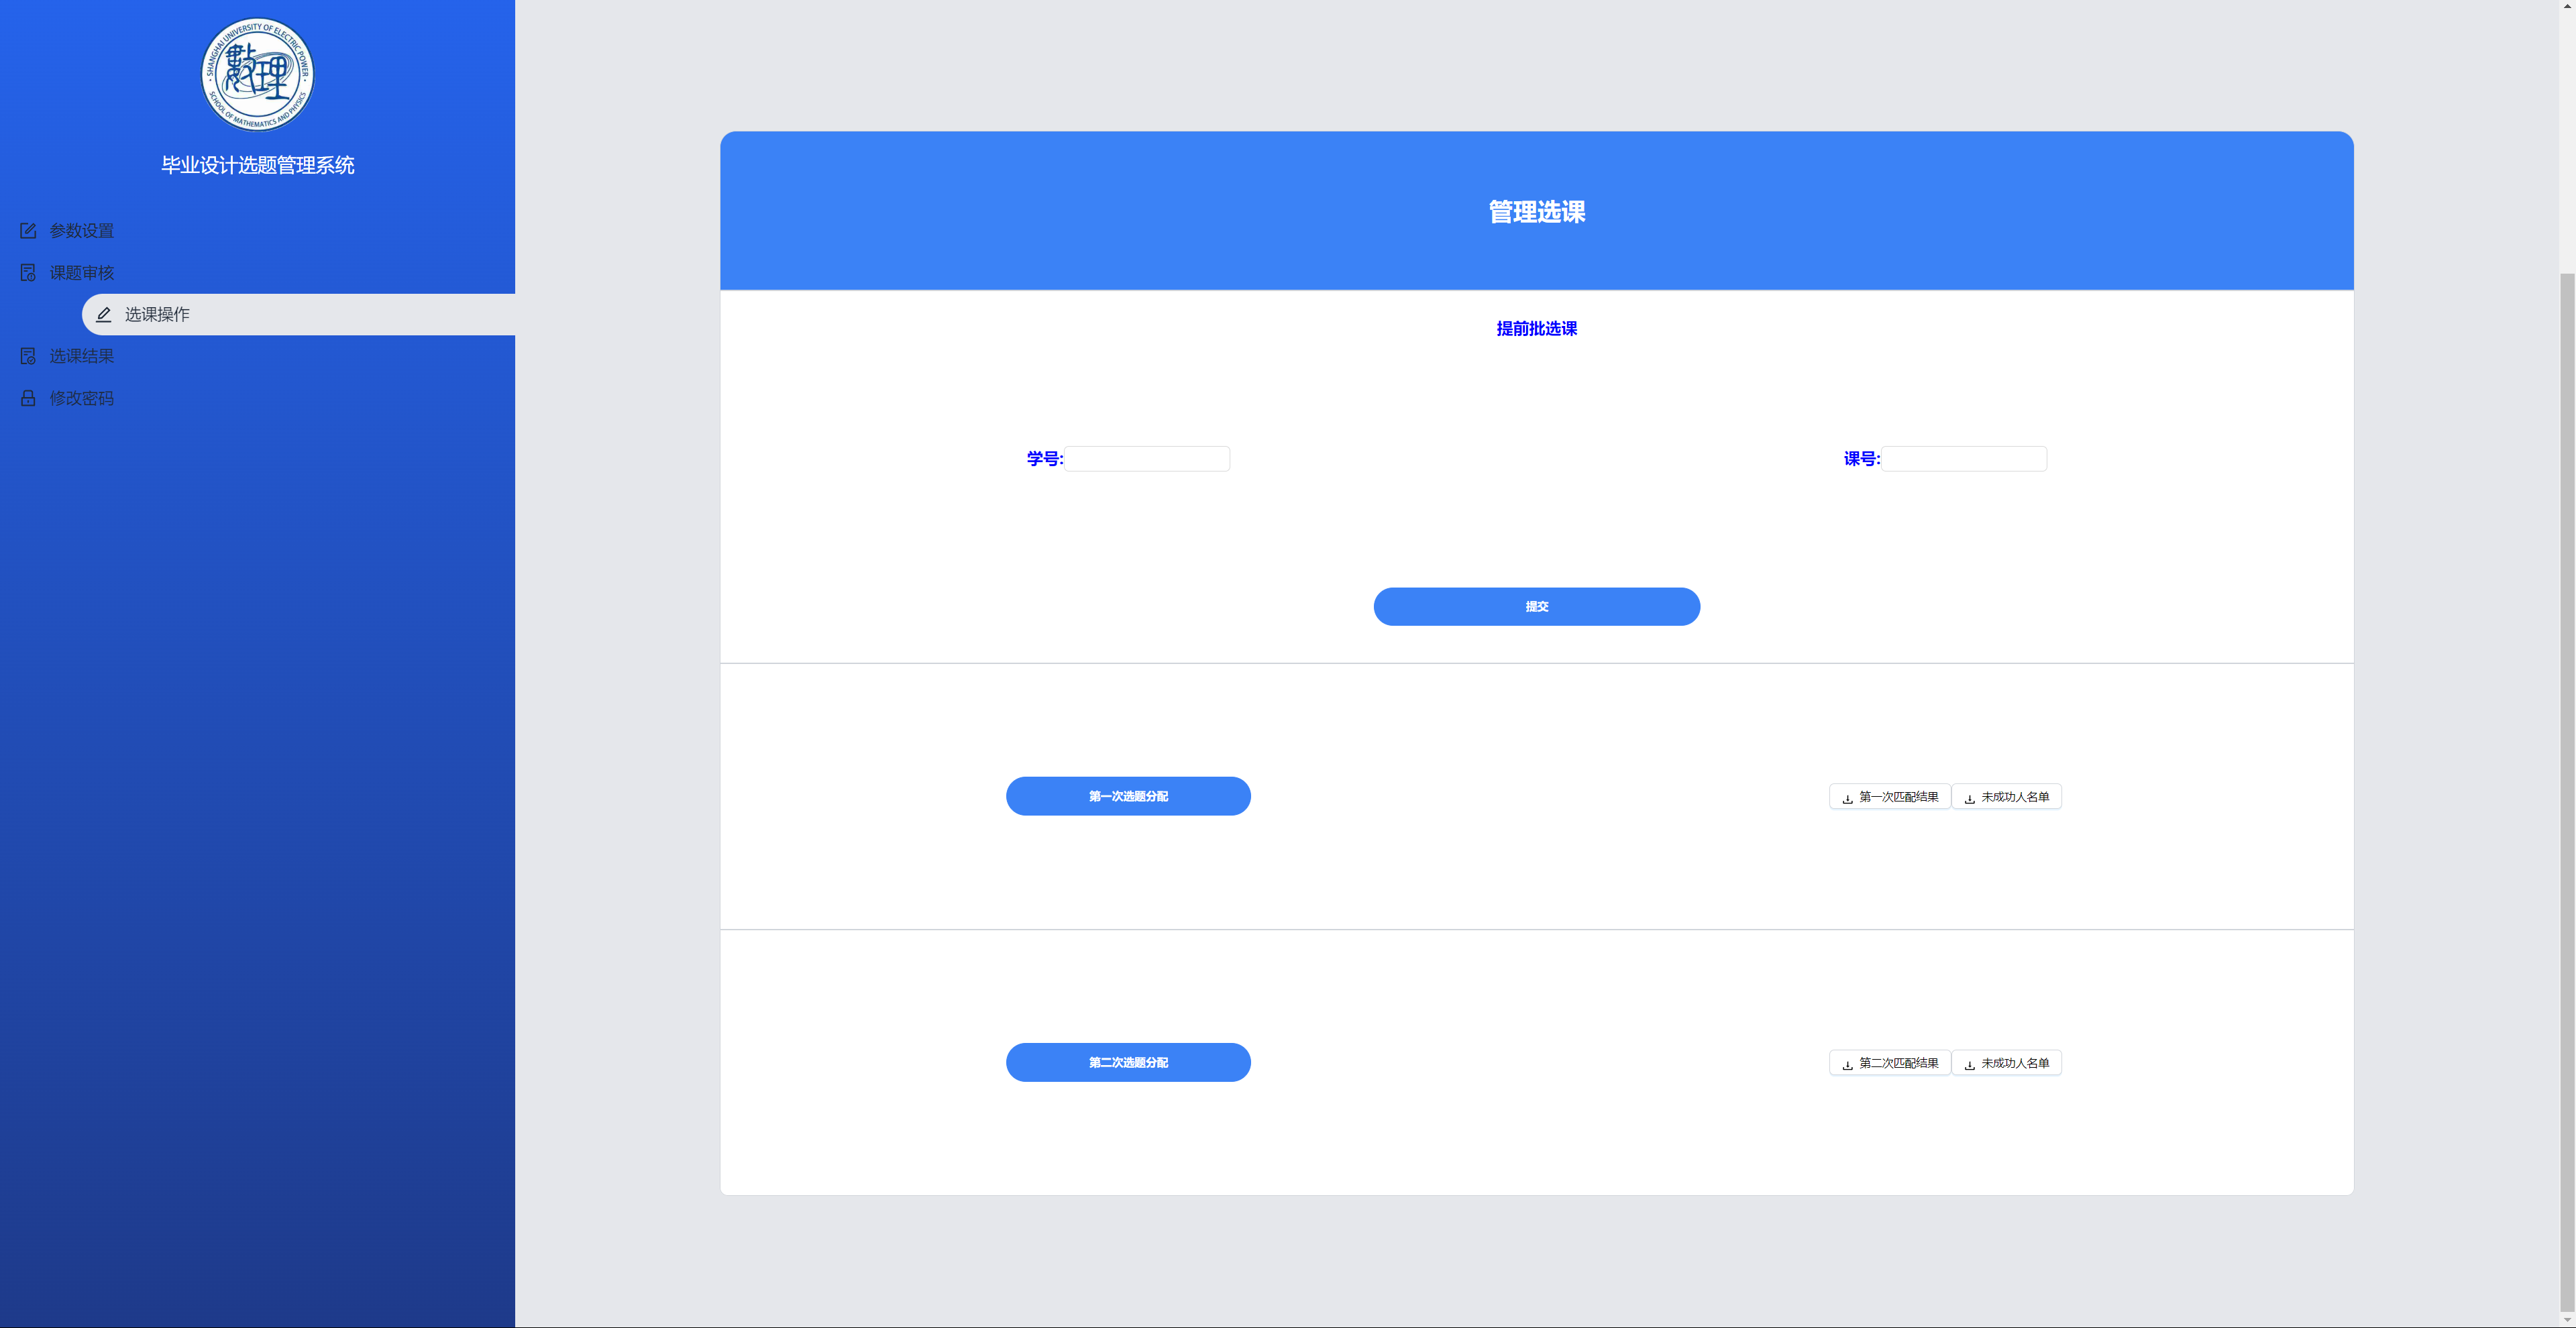
\includegraphics[width=1\textwidth]{管理员端03.png}
    \caption{管理员端-选课操作}
    \label{fig:manager03}
\end{figure}

\subsubsection{选题结果:}
在选题结果模块中,管理员可以查看学生选课的课题编号、学号、姓名、课题名称、指导老师以及学年的信息,
并且增加了按年份筛选、搜索课题和导出选课结果表格的功能;
\begin{figure}[h]
    \centering
    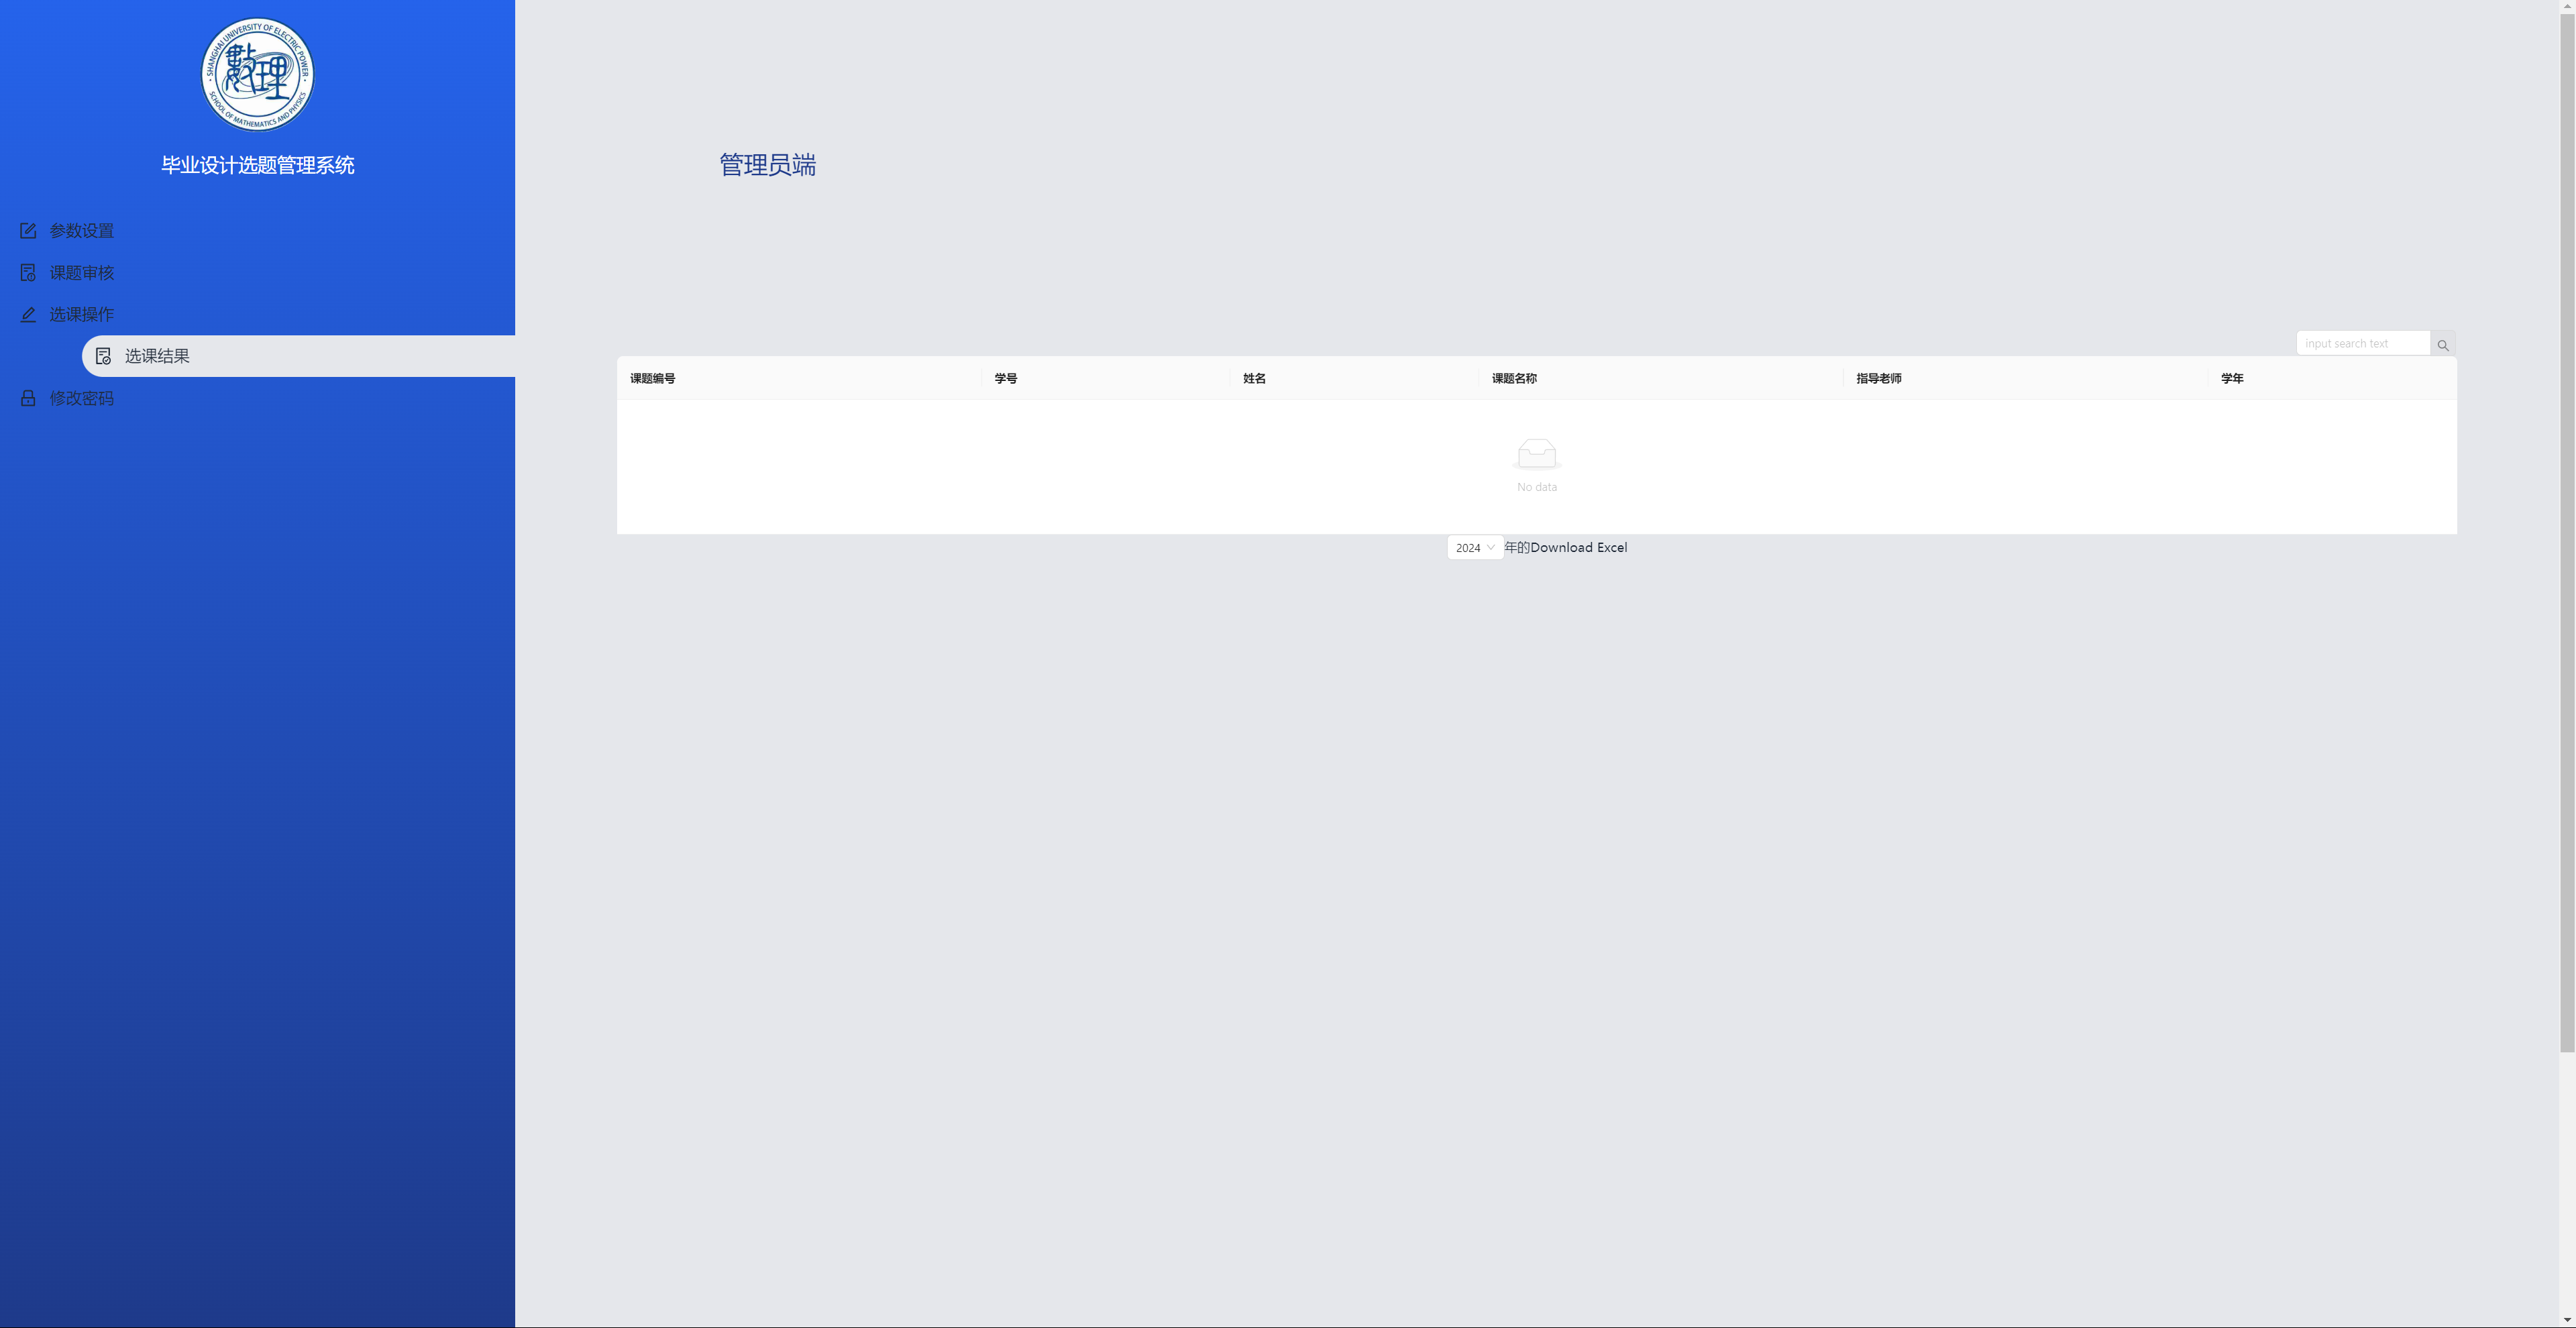
\includegraphics[width=1\textwidth]{管理员端04.png}
    \caption{管理员端-选题结果}
    \label{fig:manager04}
\end{figure}

\subsubsection{修改密码:}
最后,考虑到师生会出现忘记密码的普遍情况,
增加了修改密码这一模块用于重置教师和学生的密码。
\begin{figure}[ht]
    \centering
    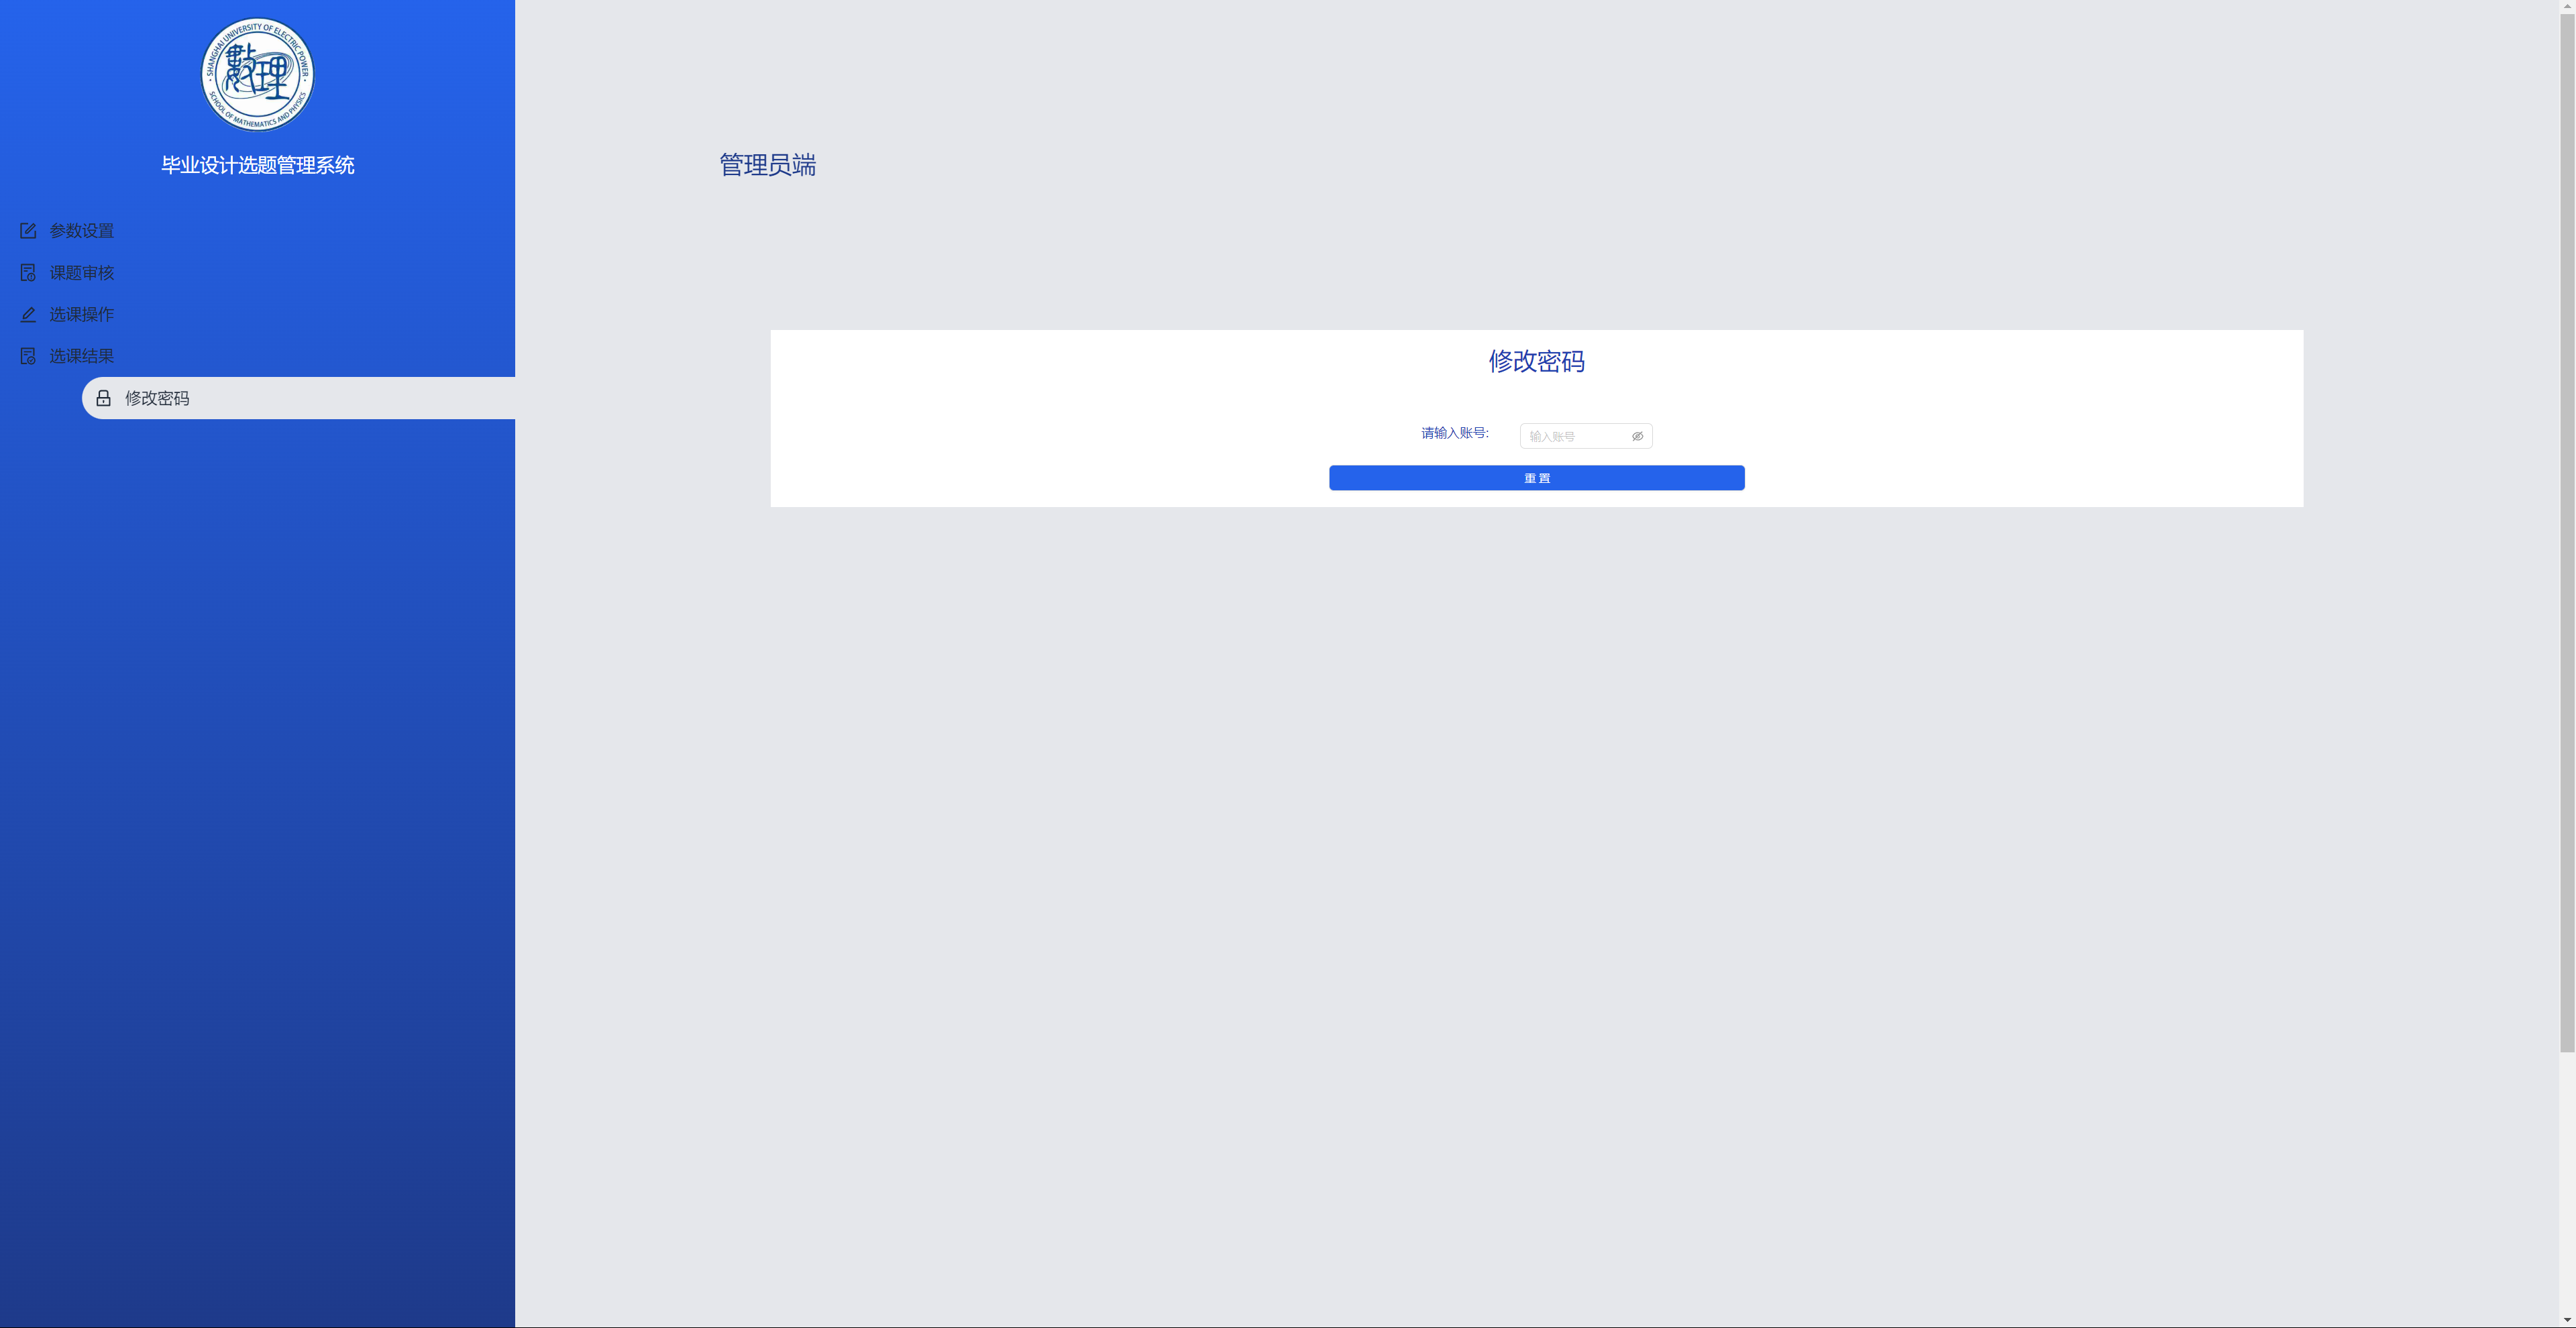
\includegraphics[width=1\textwidth]{管理员端05.png}
    \caption{管理员端-修改密码}
    \label{fig:manager05}
\end{figure}


\subsection{教师端}
\subsubsection{课题提交:}
提供教师输入课题的各项具体信息。
\begin{figure}[ht]
    \centering
    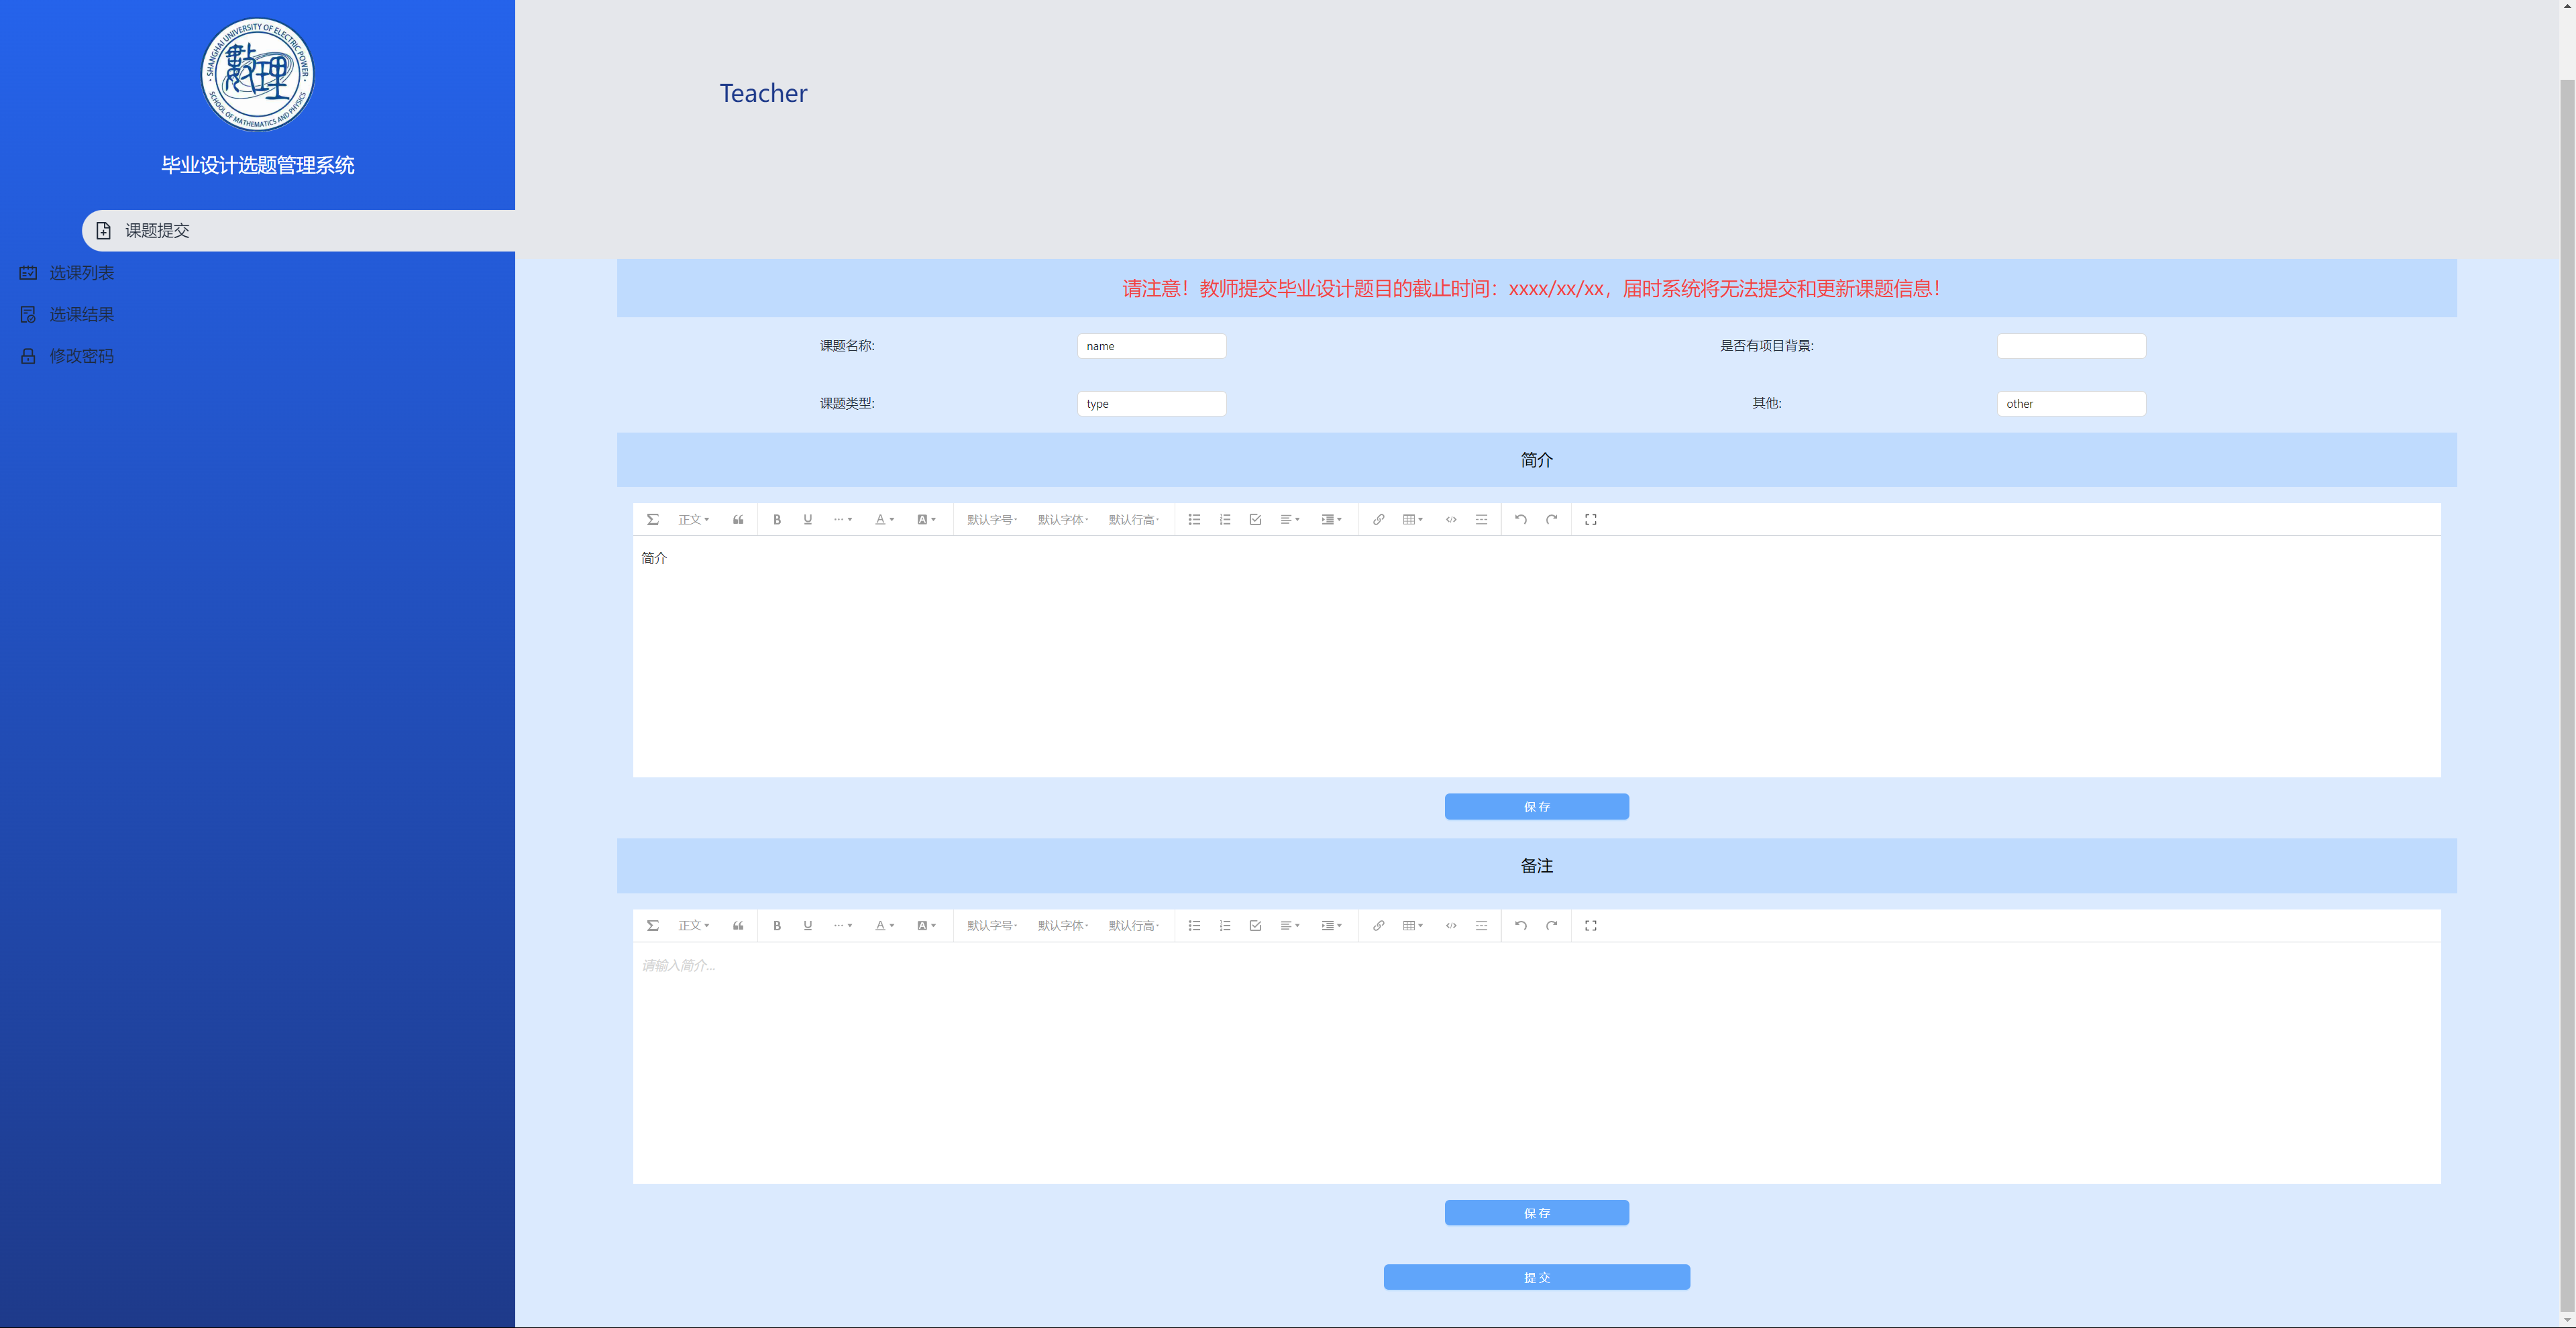
\includegraphics[width=1\textwidth]{教师端01.png}
    \caption{管理员端-课题提交}
    \label{fig:teacher01}
\end{figure}

\subsubsection{选课列表:}
查看提交的课题的信息并进行修改删除等操作。
\begin{figure}[ht]
    \centering
    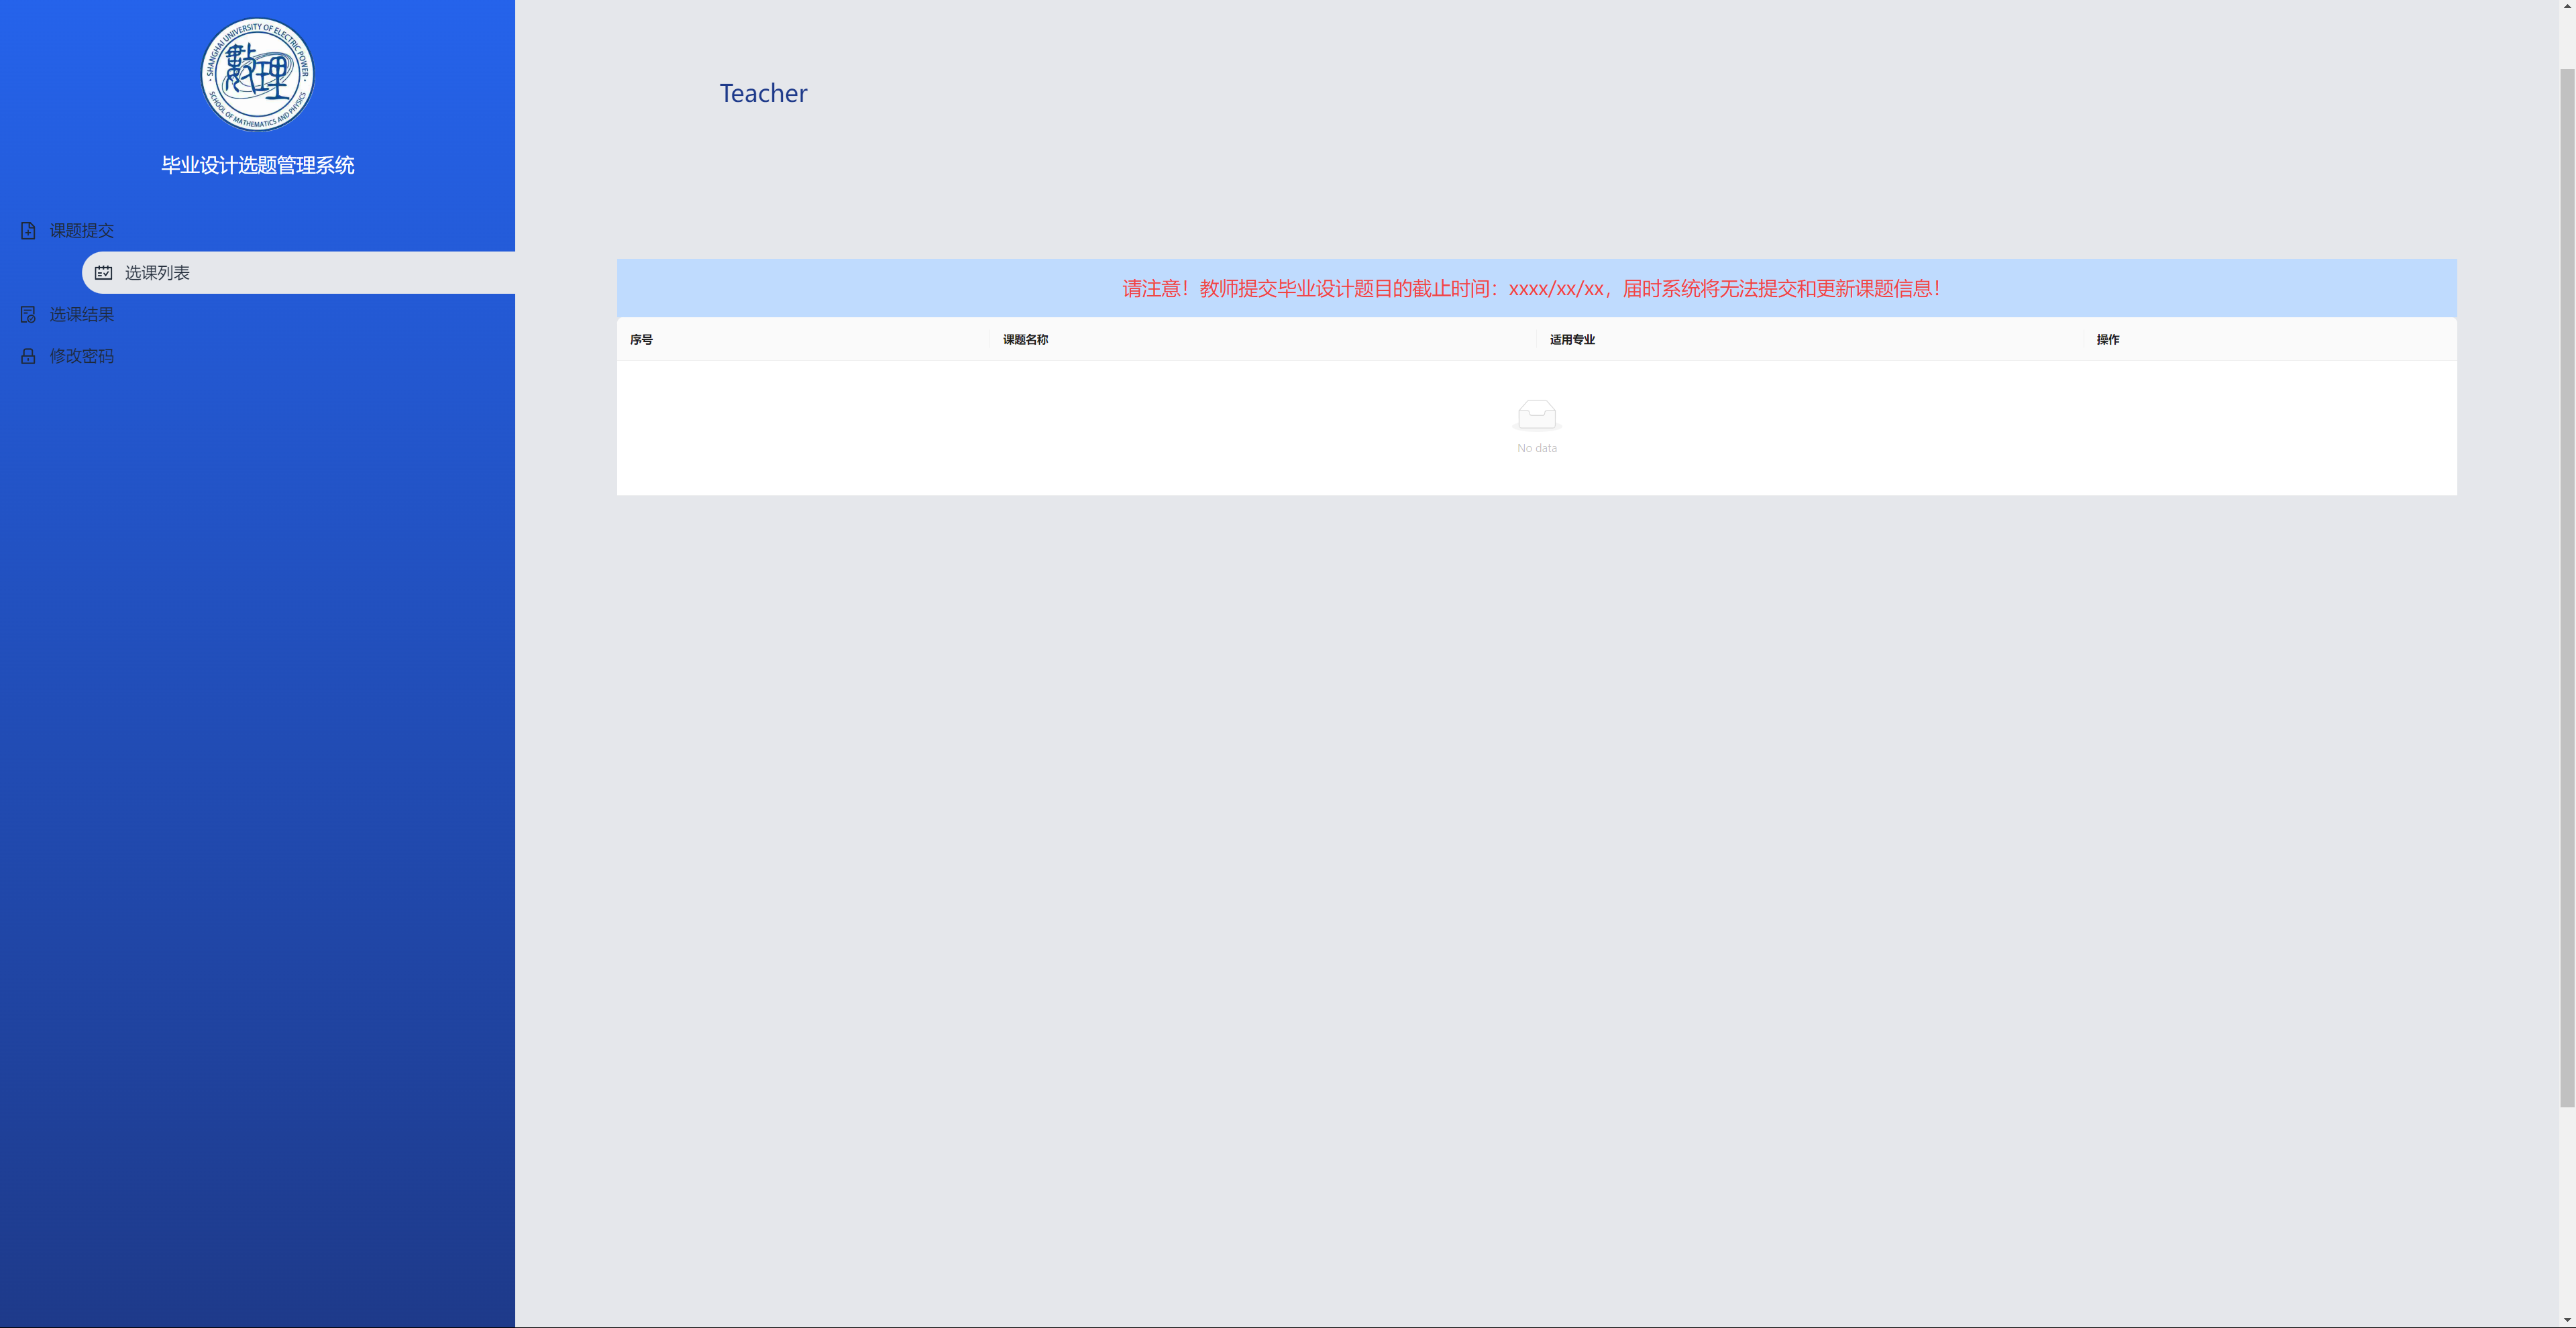
\includegraphics[width=1\textwidth]{教师端02.png}
    \caption{教师端-选课列表}
    \label{fig:teacher02}
\end{figure}

\subsubsection{选课结果:}
查看学生的选题结果信息,
包括学生姓名学号专业班级联系方式,
便于老师了解自己课题的选题情况。
\begin{figure}[ht]
    \centering
    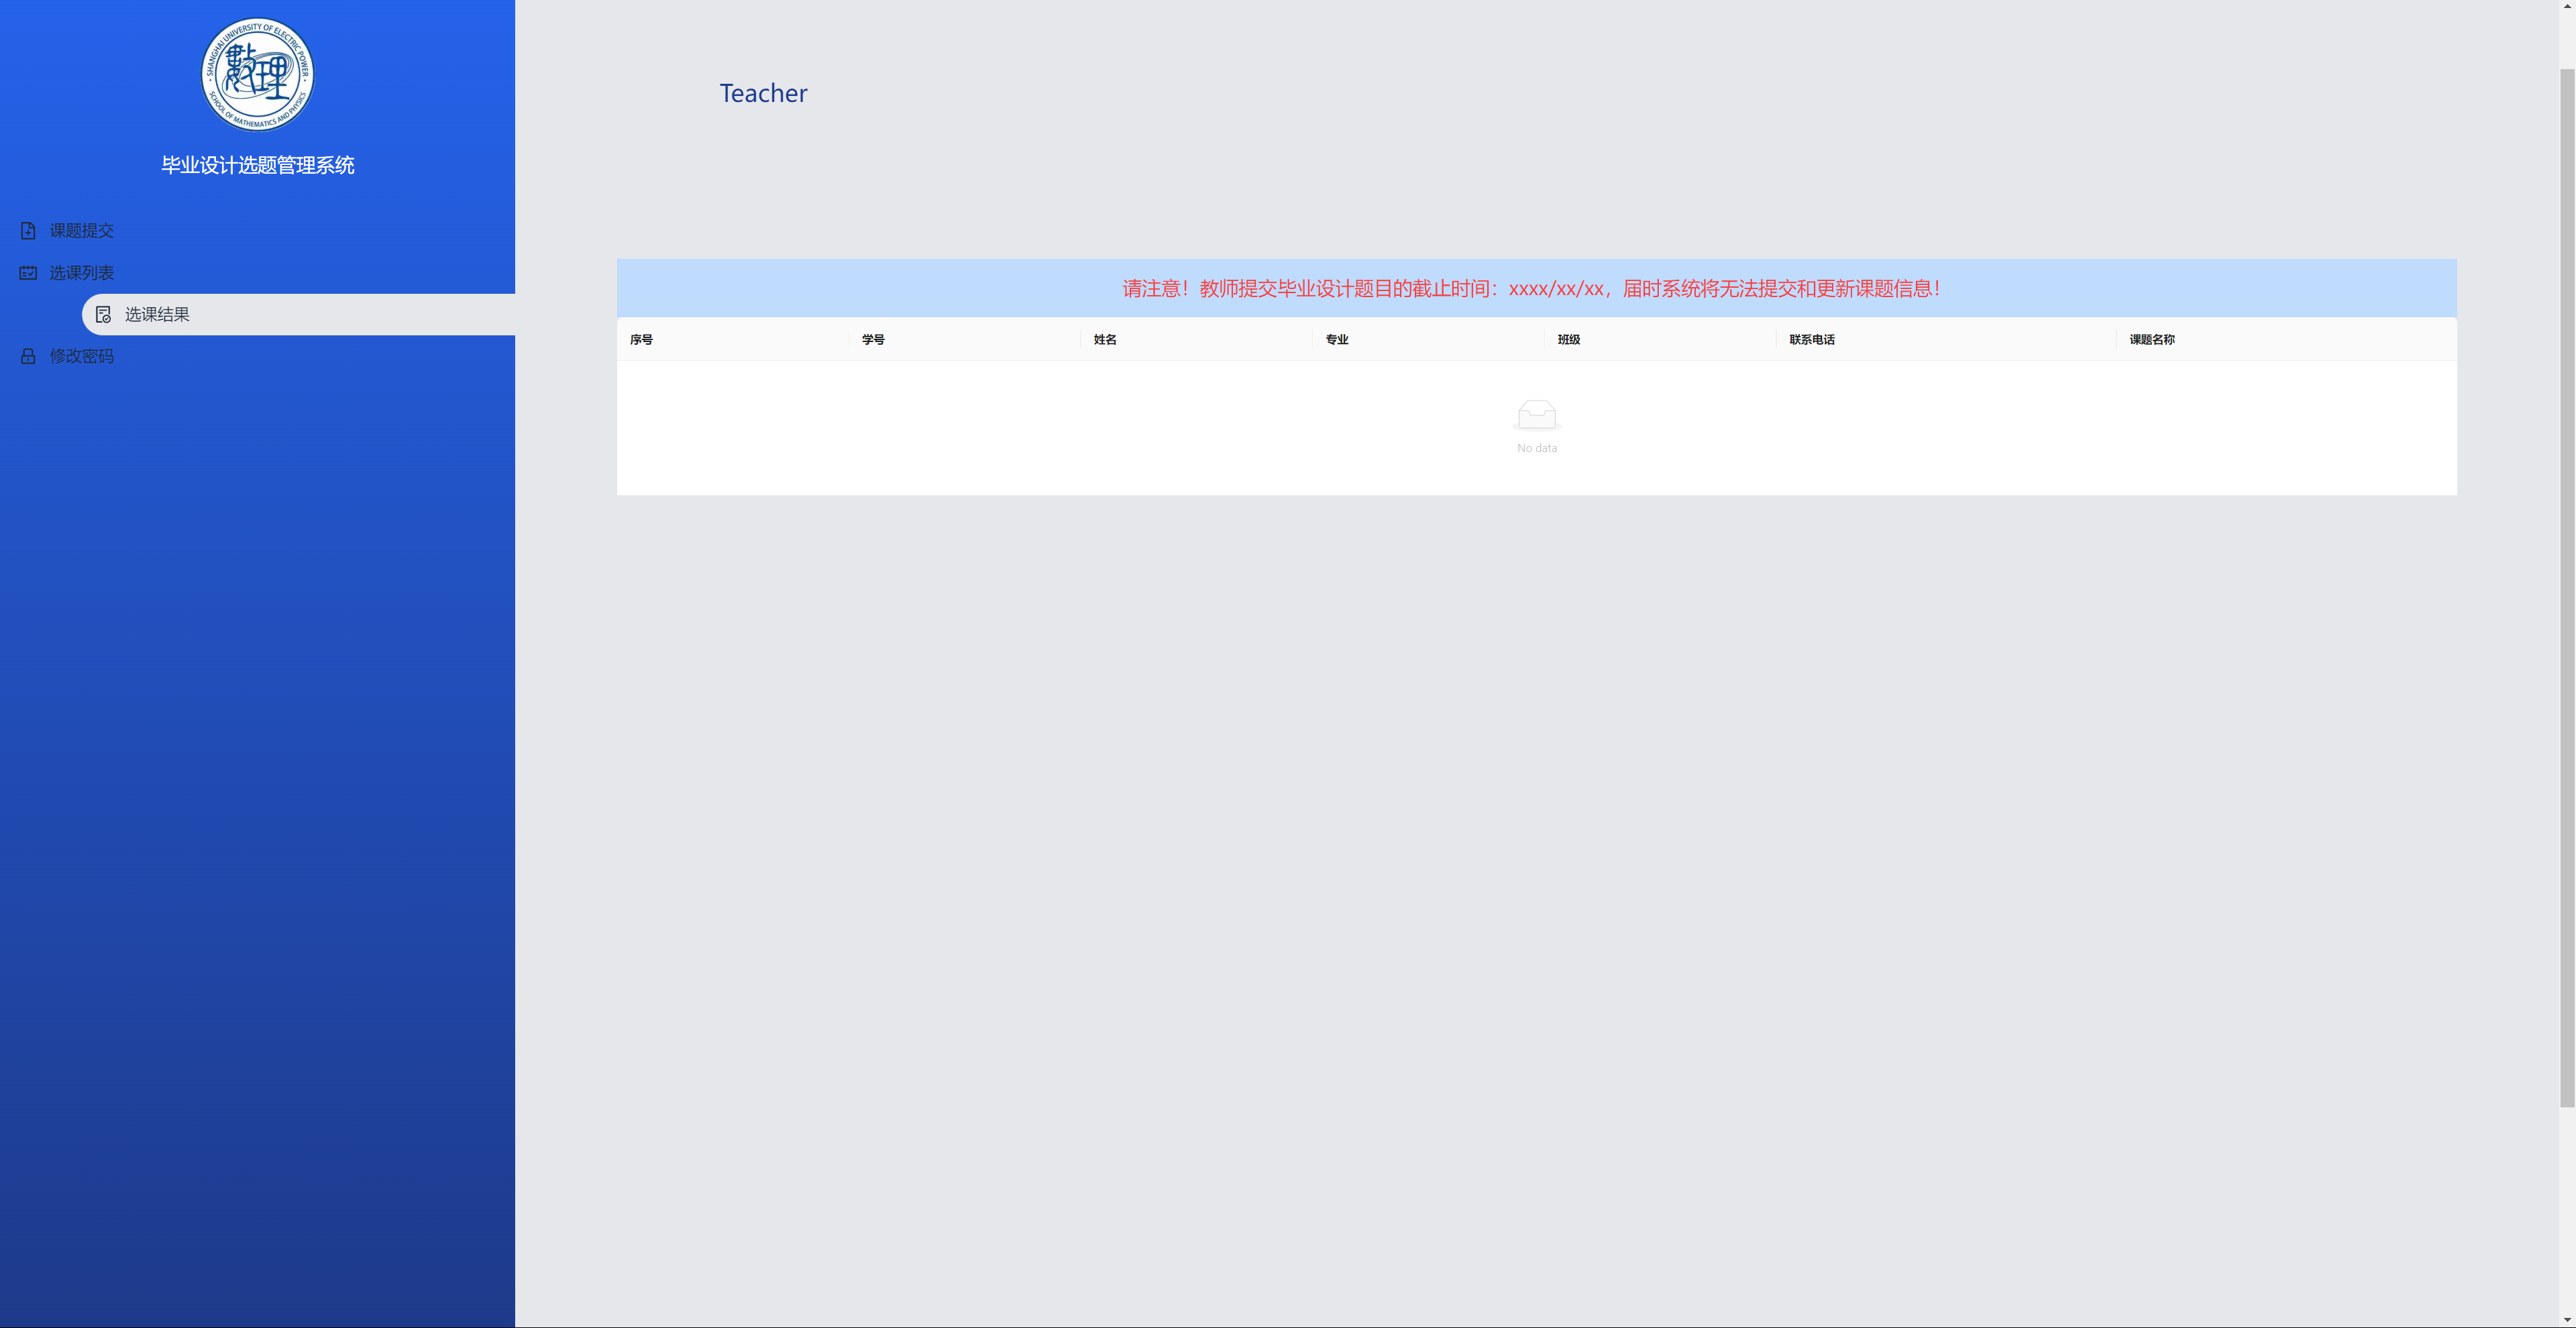
\includegraphics[width=1\textwidth]{教师端03.png}
    \caption{教师端-选课结果}
    \label{fig:teacher03}
\end{figure}

\subsubsection{修改密码:}
提供了教师更新密码的窗口。
\begin{figure}[ht]
    \centering
    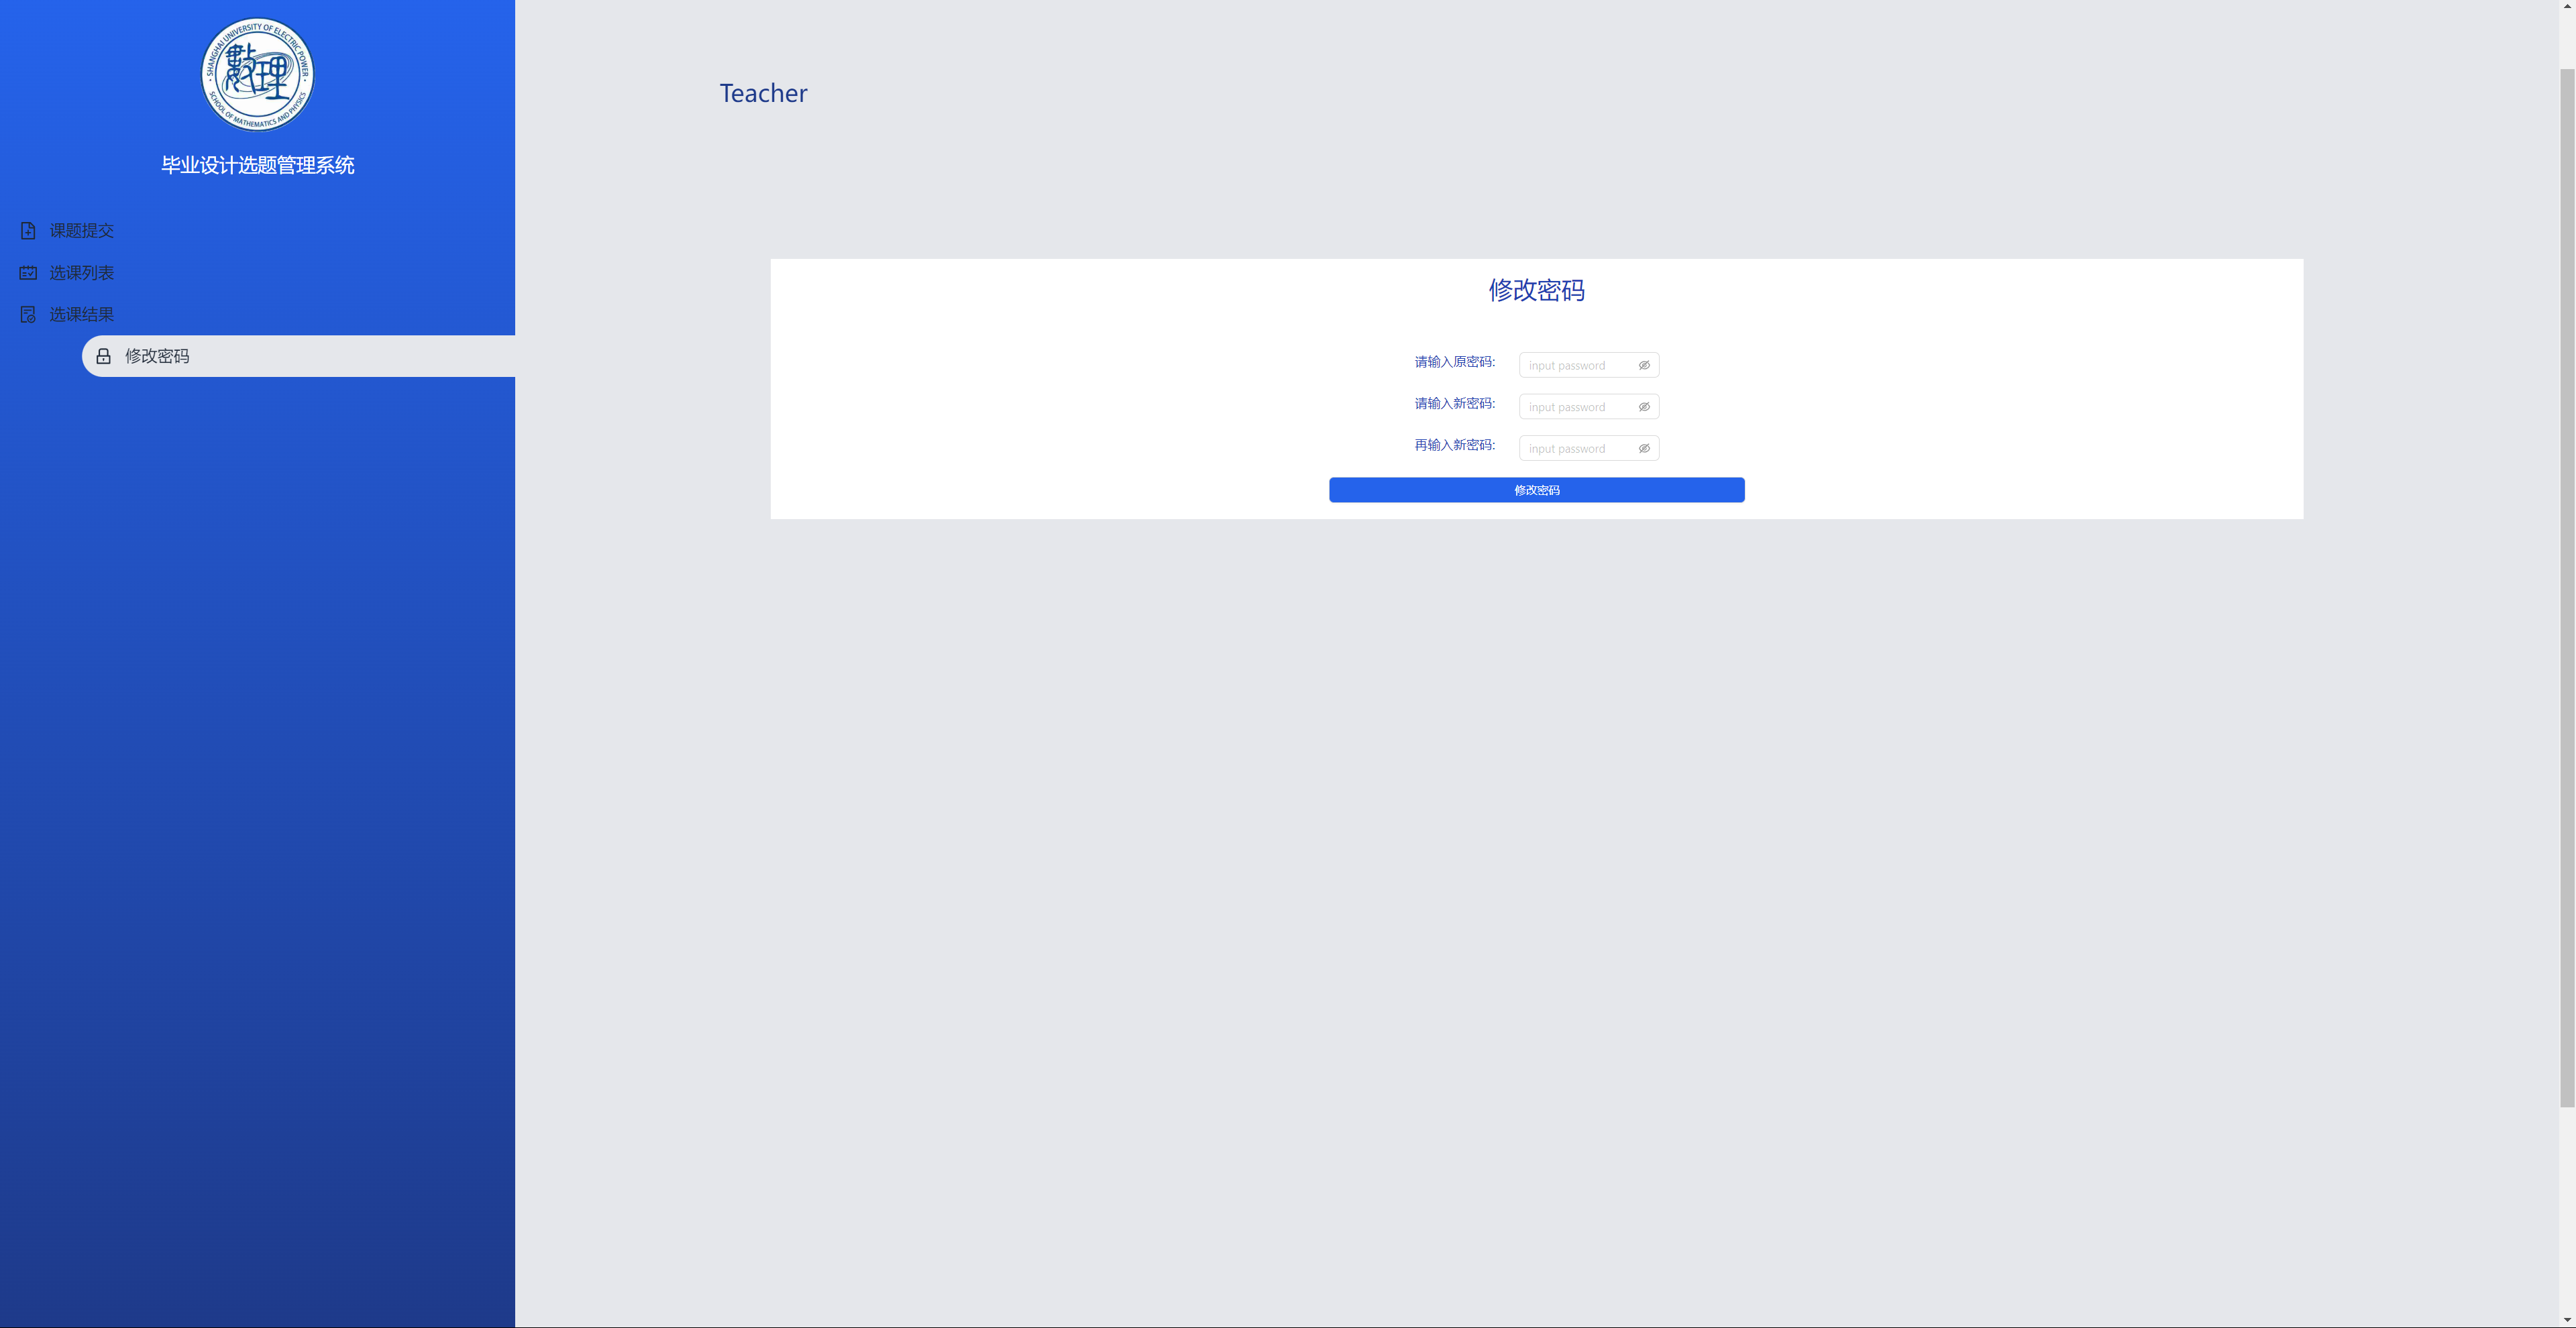
\includegraphics[width=1\textwidth]{教师端04.png}
    \caption{教师端-修改密码}
    \label{fig:teacher04}
\end{figure}


\subsection{普通用户端}
\subsubsection{选题规则:}
在这里学生可以查看数理学院毕业论文(设计)选题规则。
\begin{figure}[h]
    \centering
    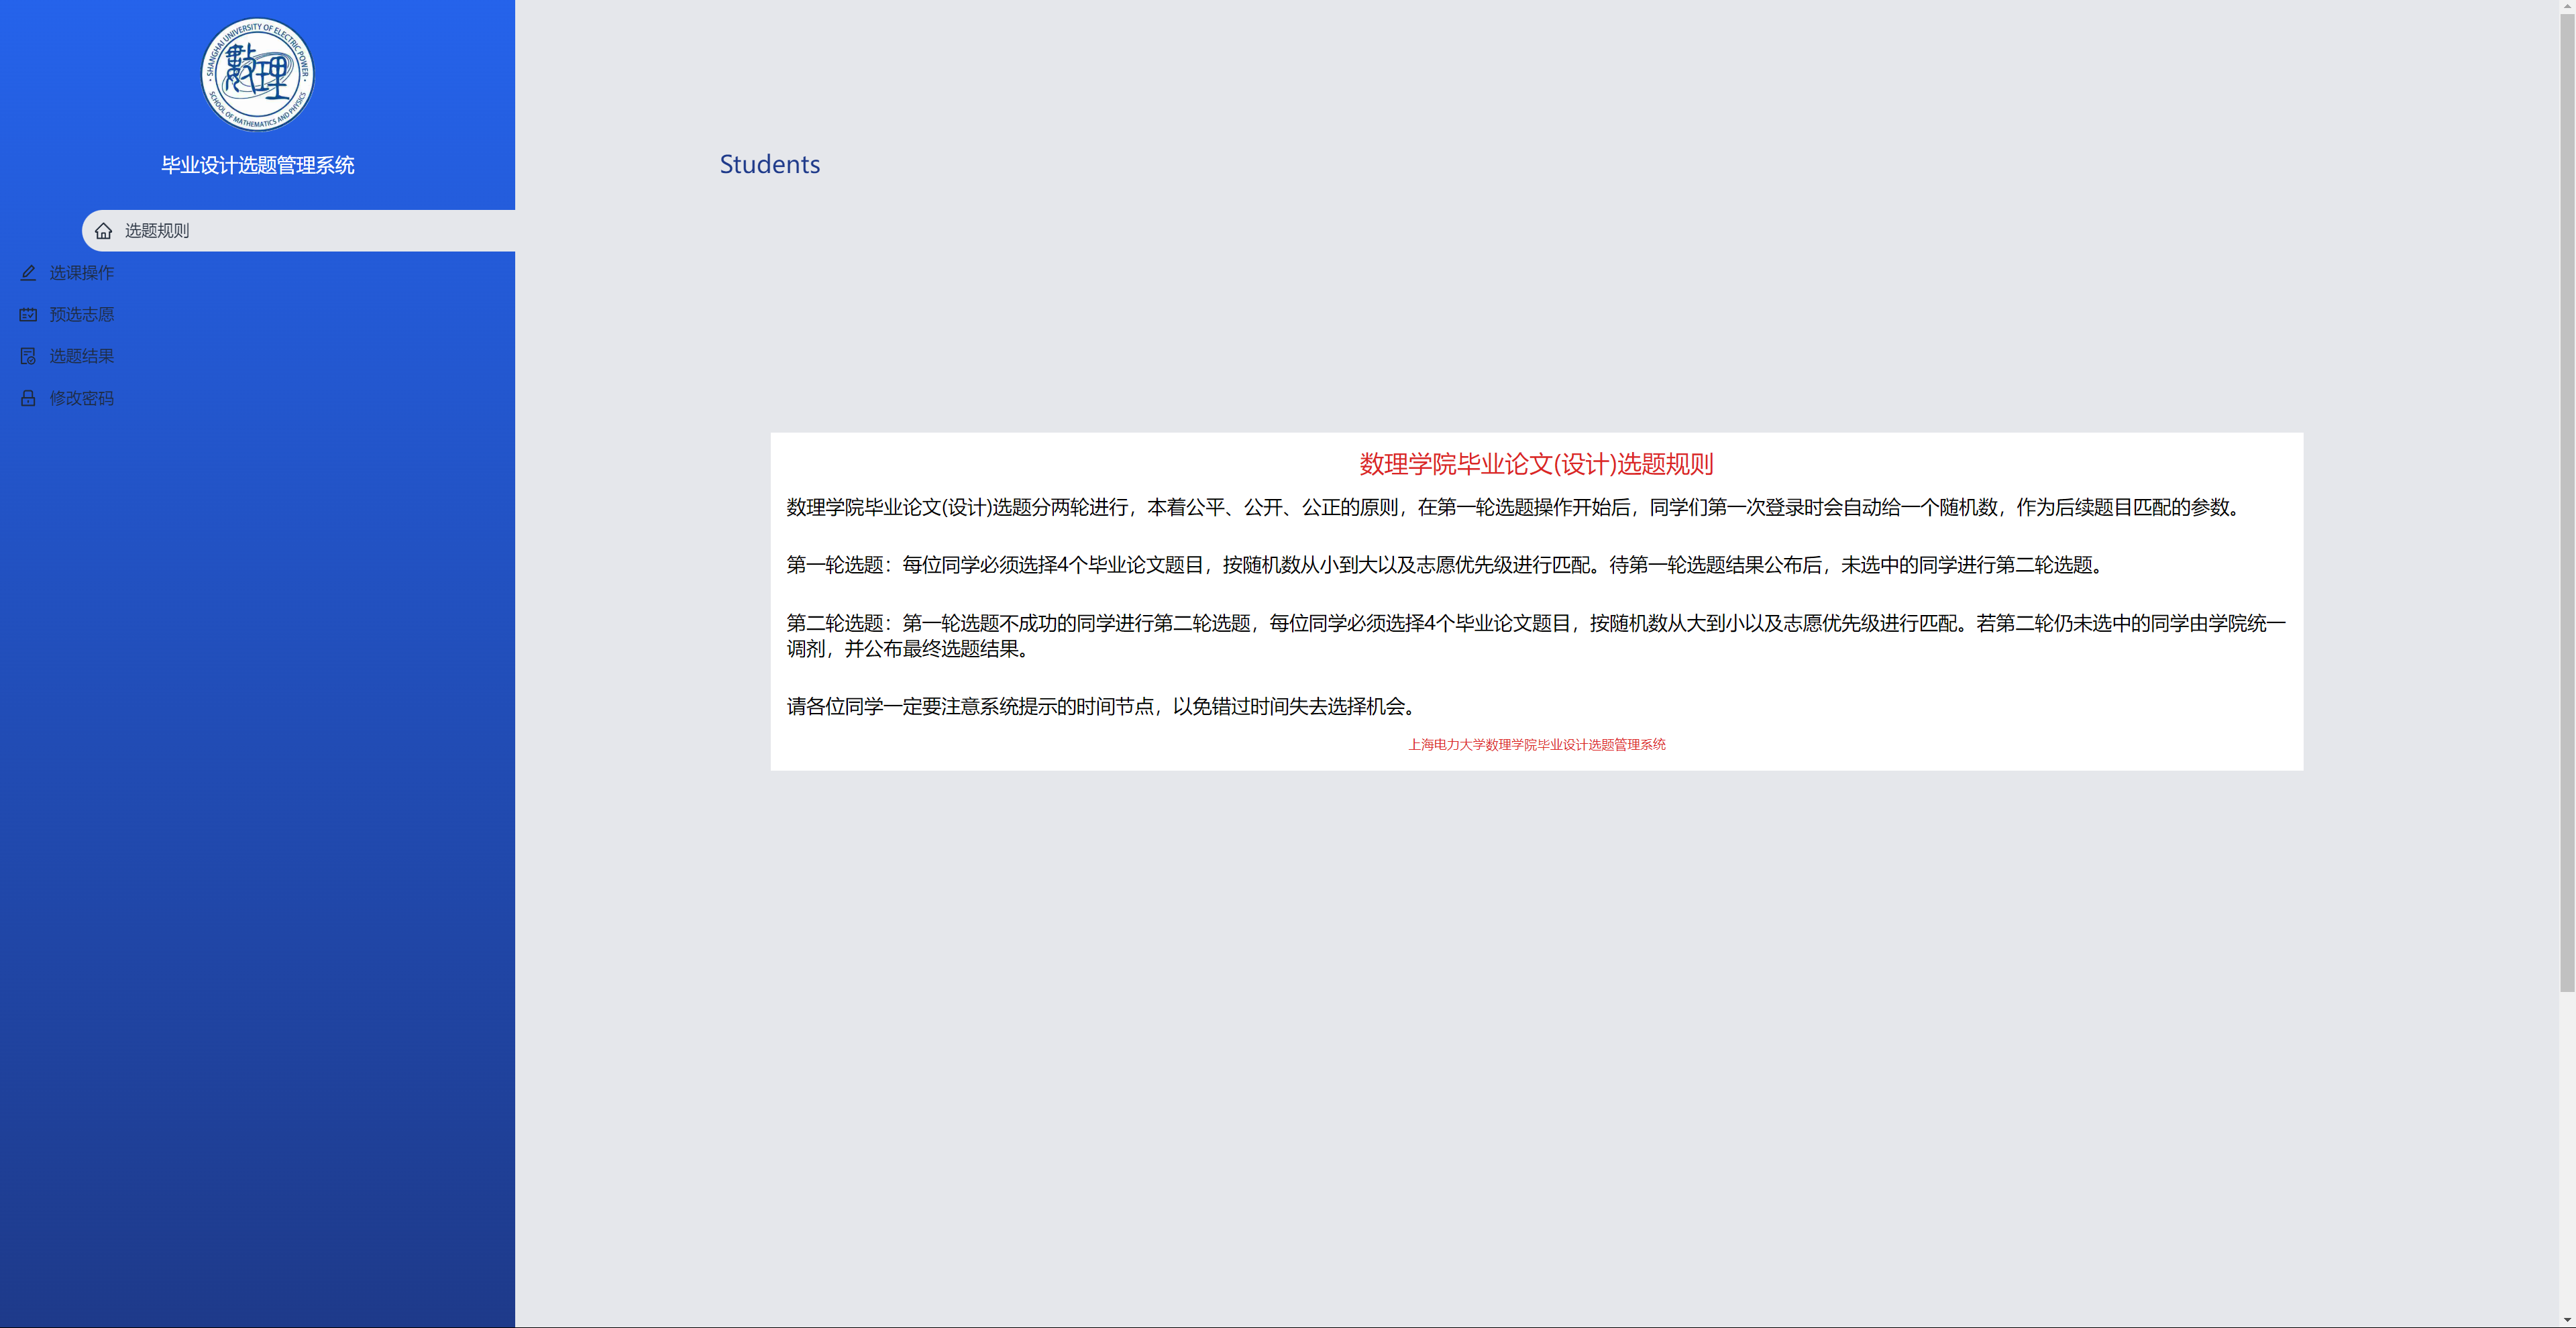
\includegraphics[width=1\textwidth]{学生端01.png}
    \caption{学生端-选题规则}
    \label{fig:student01}
\end{figure}

\subsubsection{选课操作:}
在学生端的选课操作模块中,学生可以查看课题的编号、名称以及类别进行选题操作。
\begin{figure}[h]
    \centering
    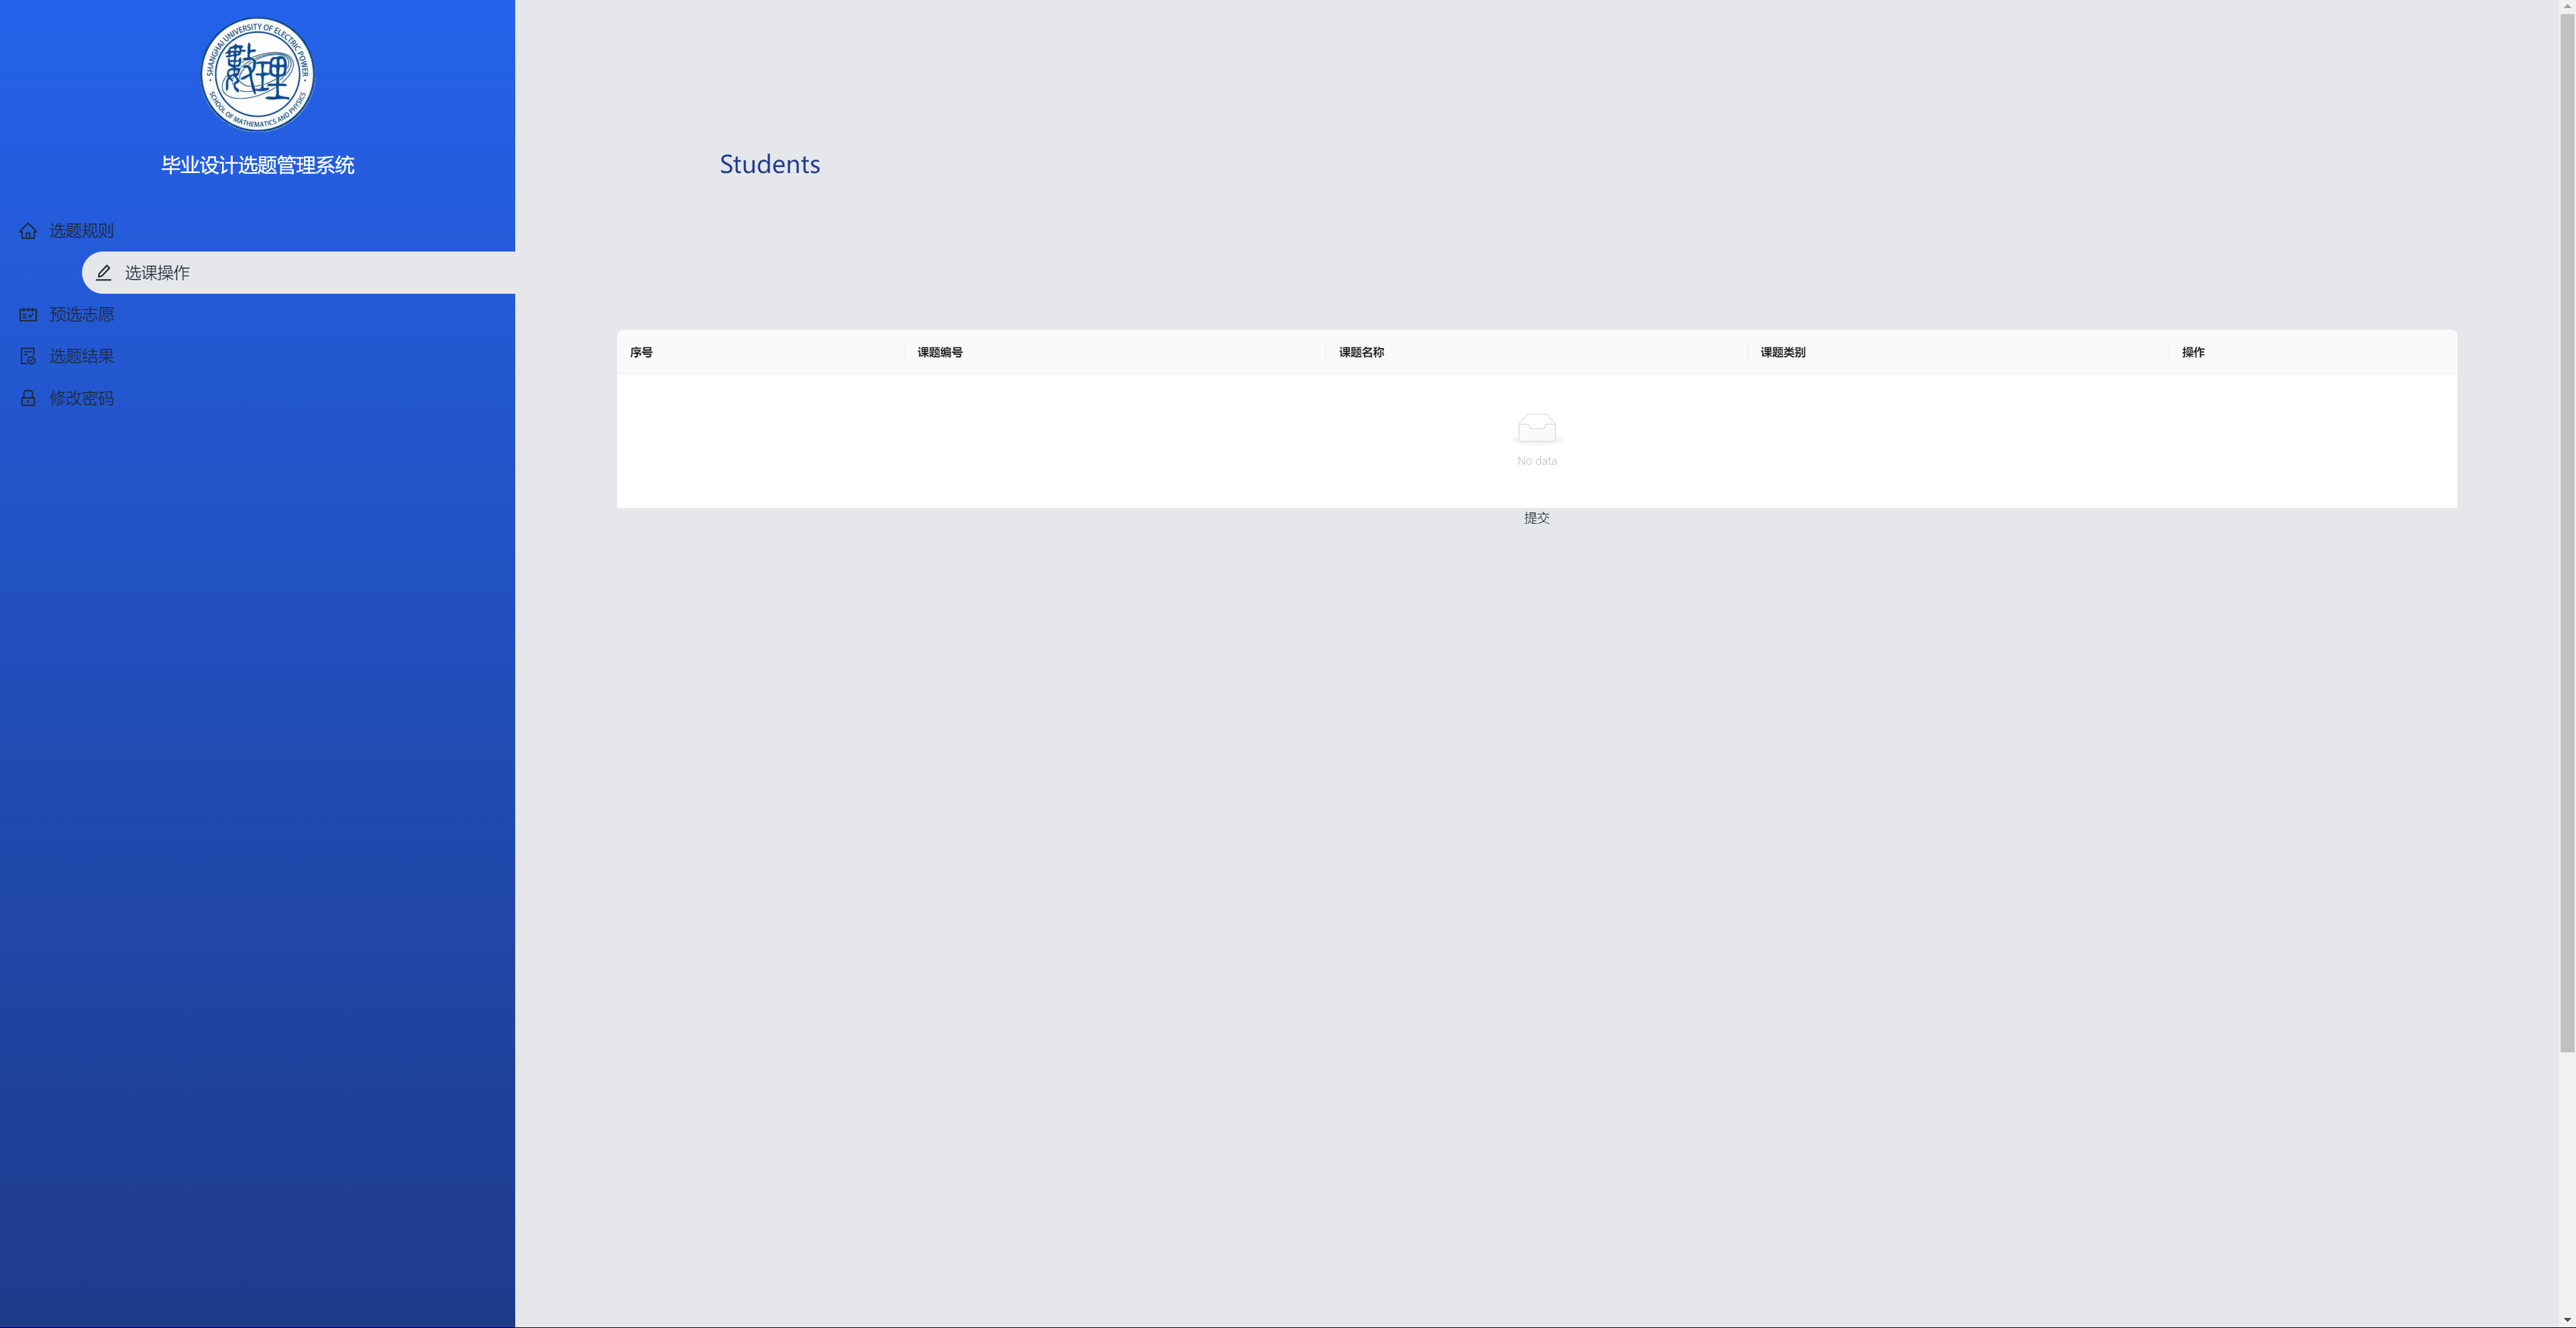
\includegraphics[width=1\textwidth]{学生端02.png}
    \caption{学生端-选课操作}
    \label{fig:student02}
\end{figure}

\clearpage

\subsubsection{预选志愿:}
在预选志愿界面,学生可以查看自己预选的第一到第四志愿,以及对应课题的信息。
\begin{figure}[h]
    \centering
    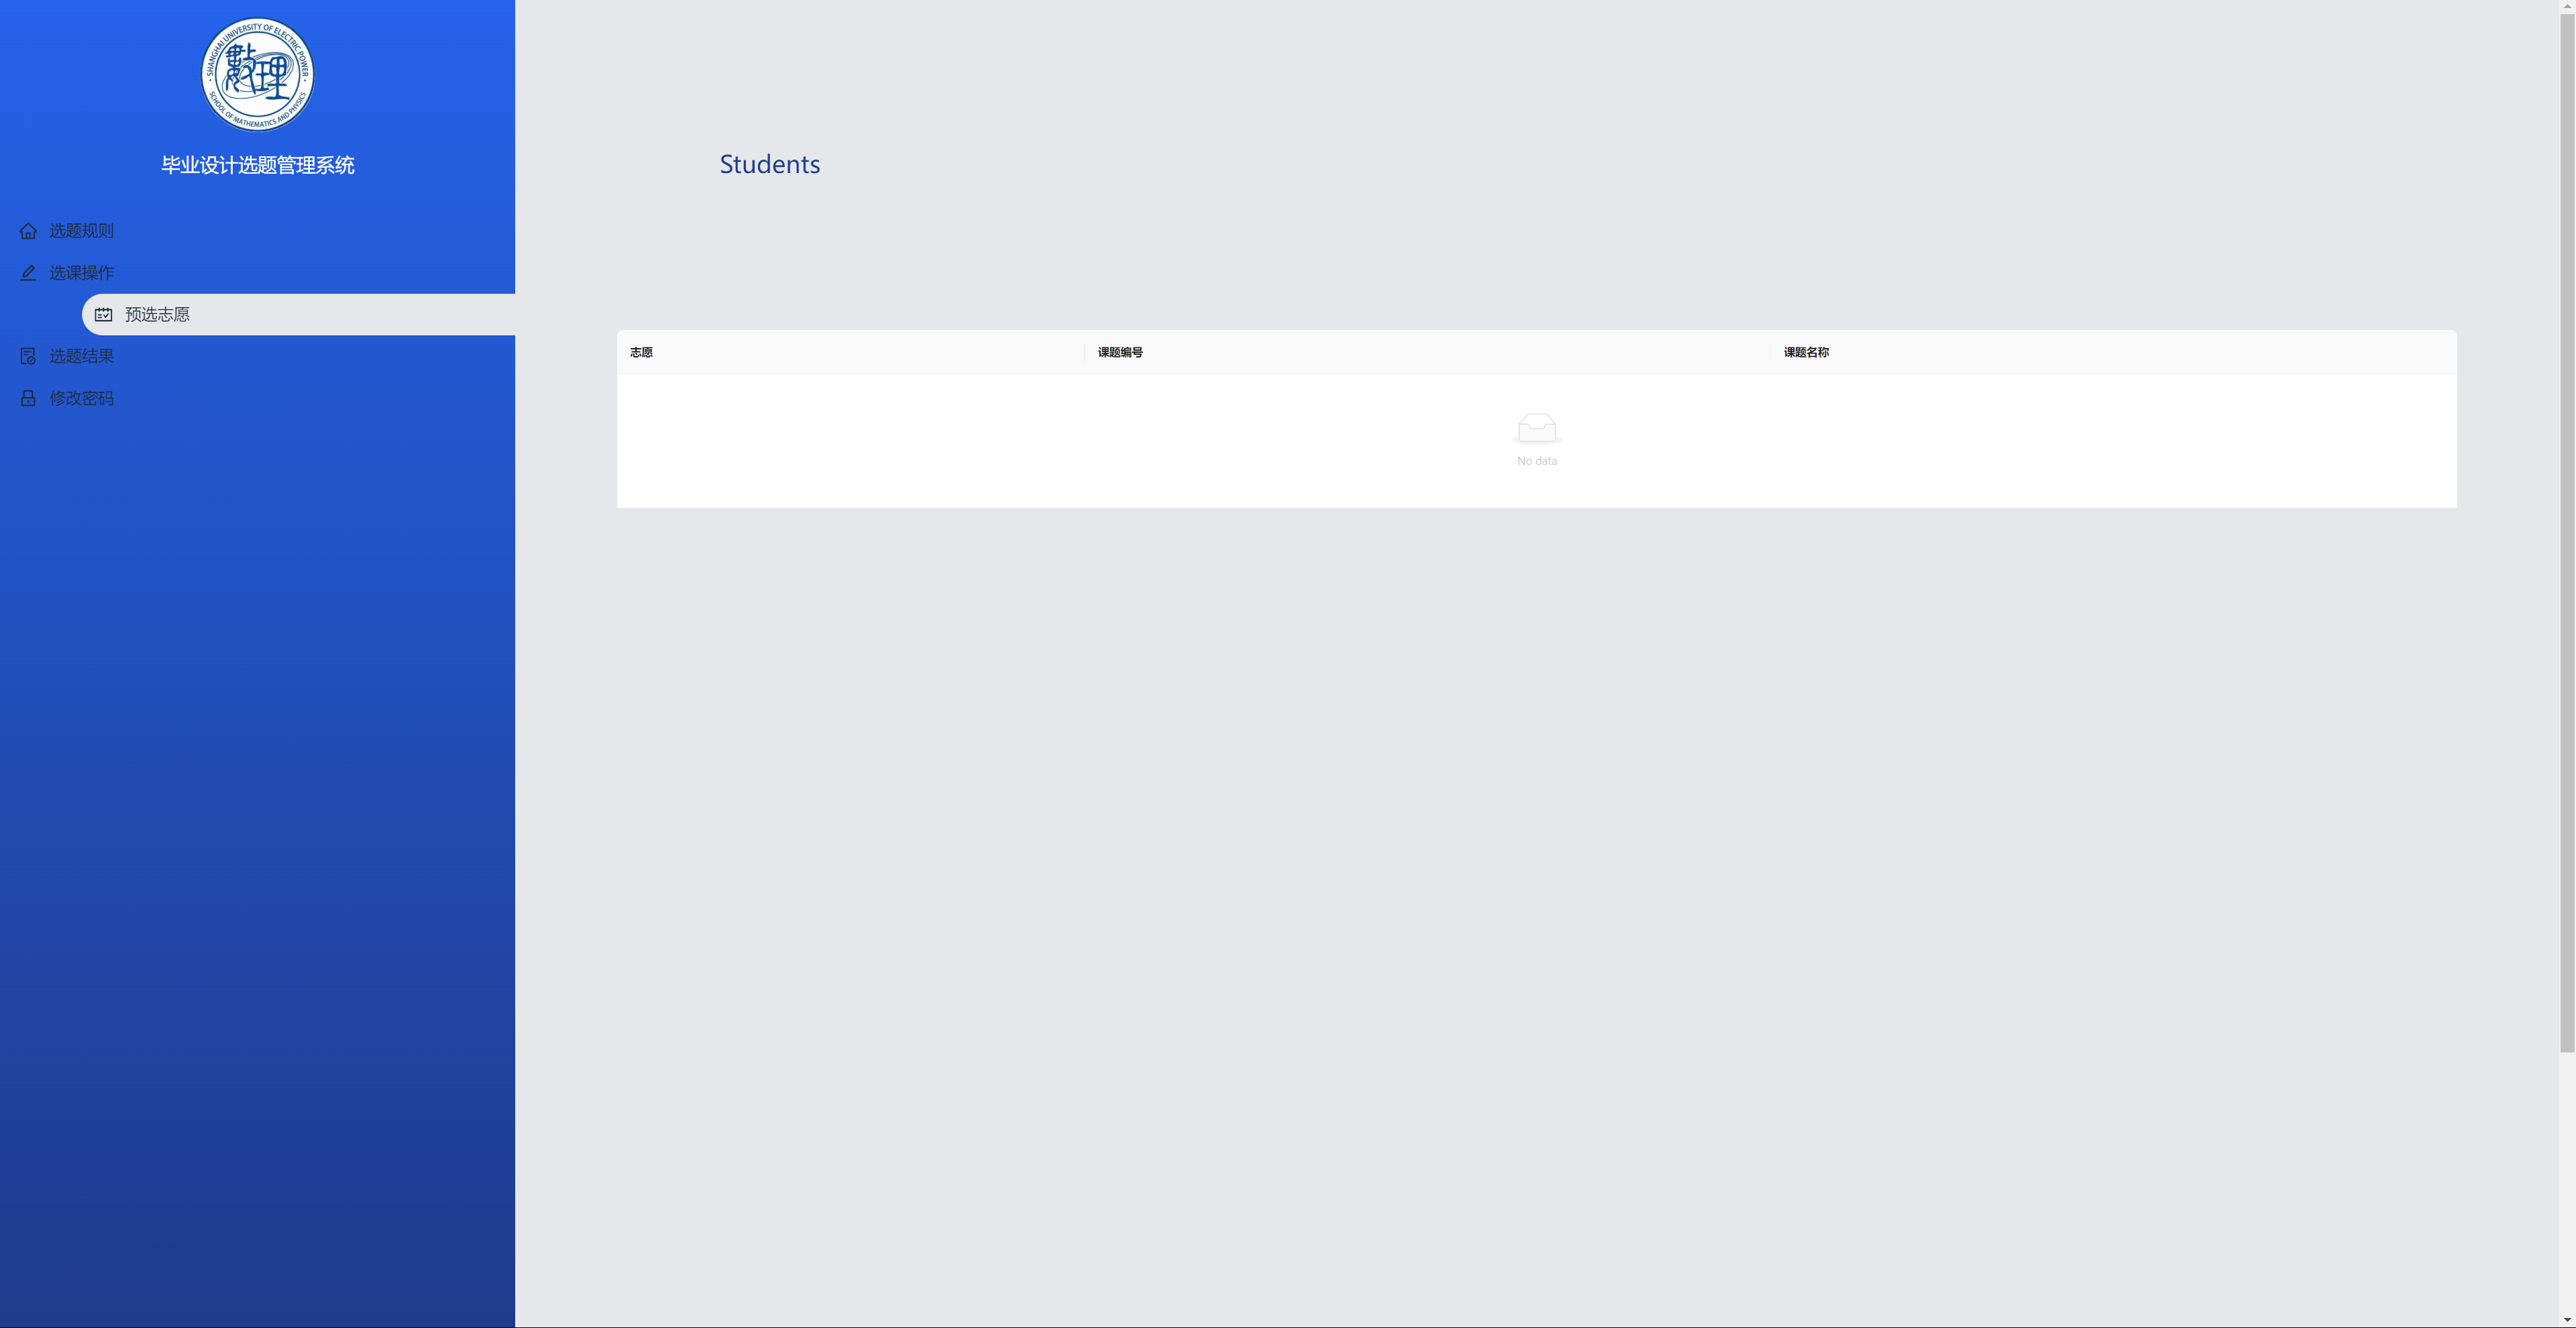
\includegraphics[width=1\textwidth]{学生端03.png}
    \caption{学生端-预选志愿}
    \label{fig:student03}
\end{figure}

\subsubsection{选题结果:}
在选题结果模块中,学生可以查看自己最后选择到的课题的课题编号、名称信息,
并且可以查看自己课题的指导老师。
\begin{figure}[h]
    \centering
    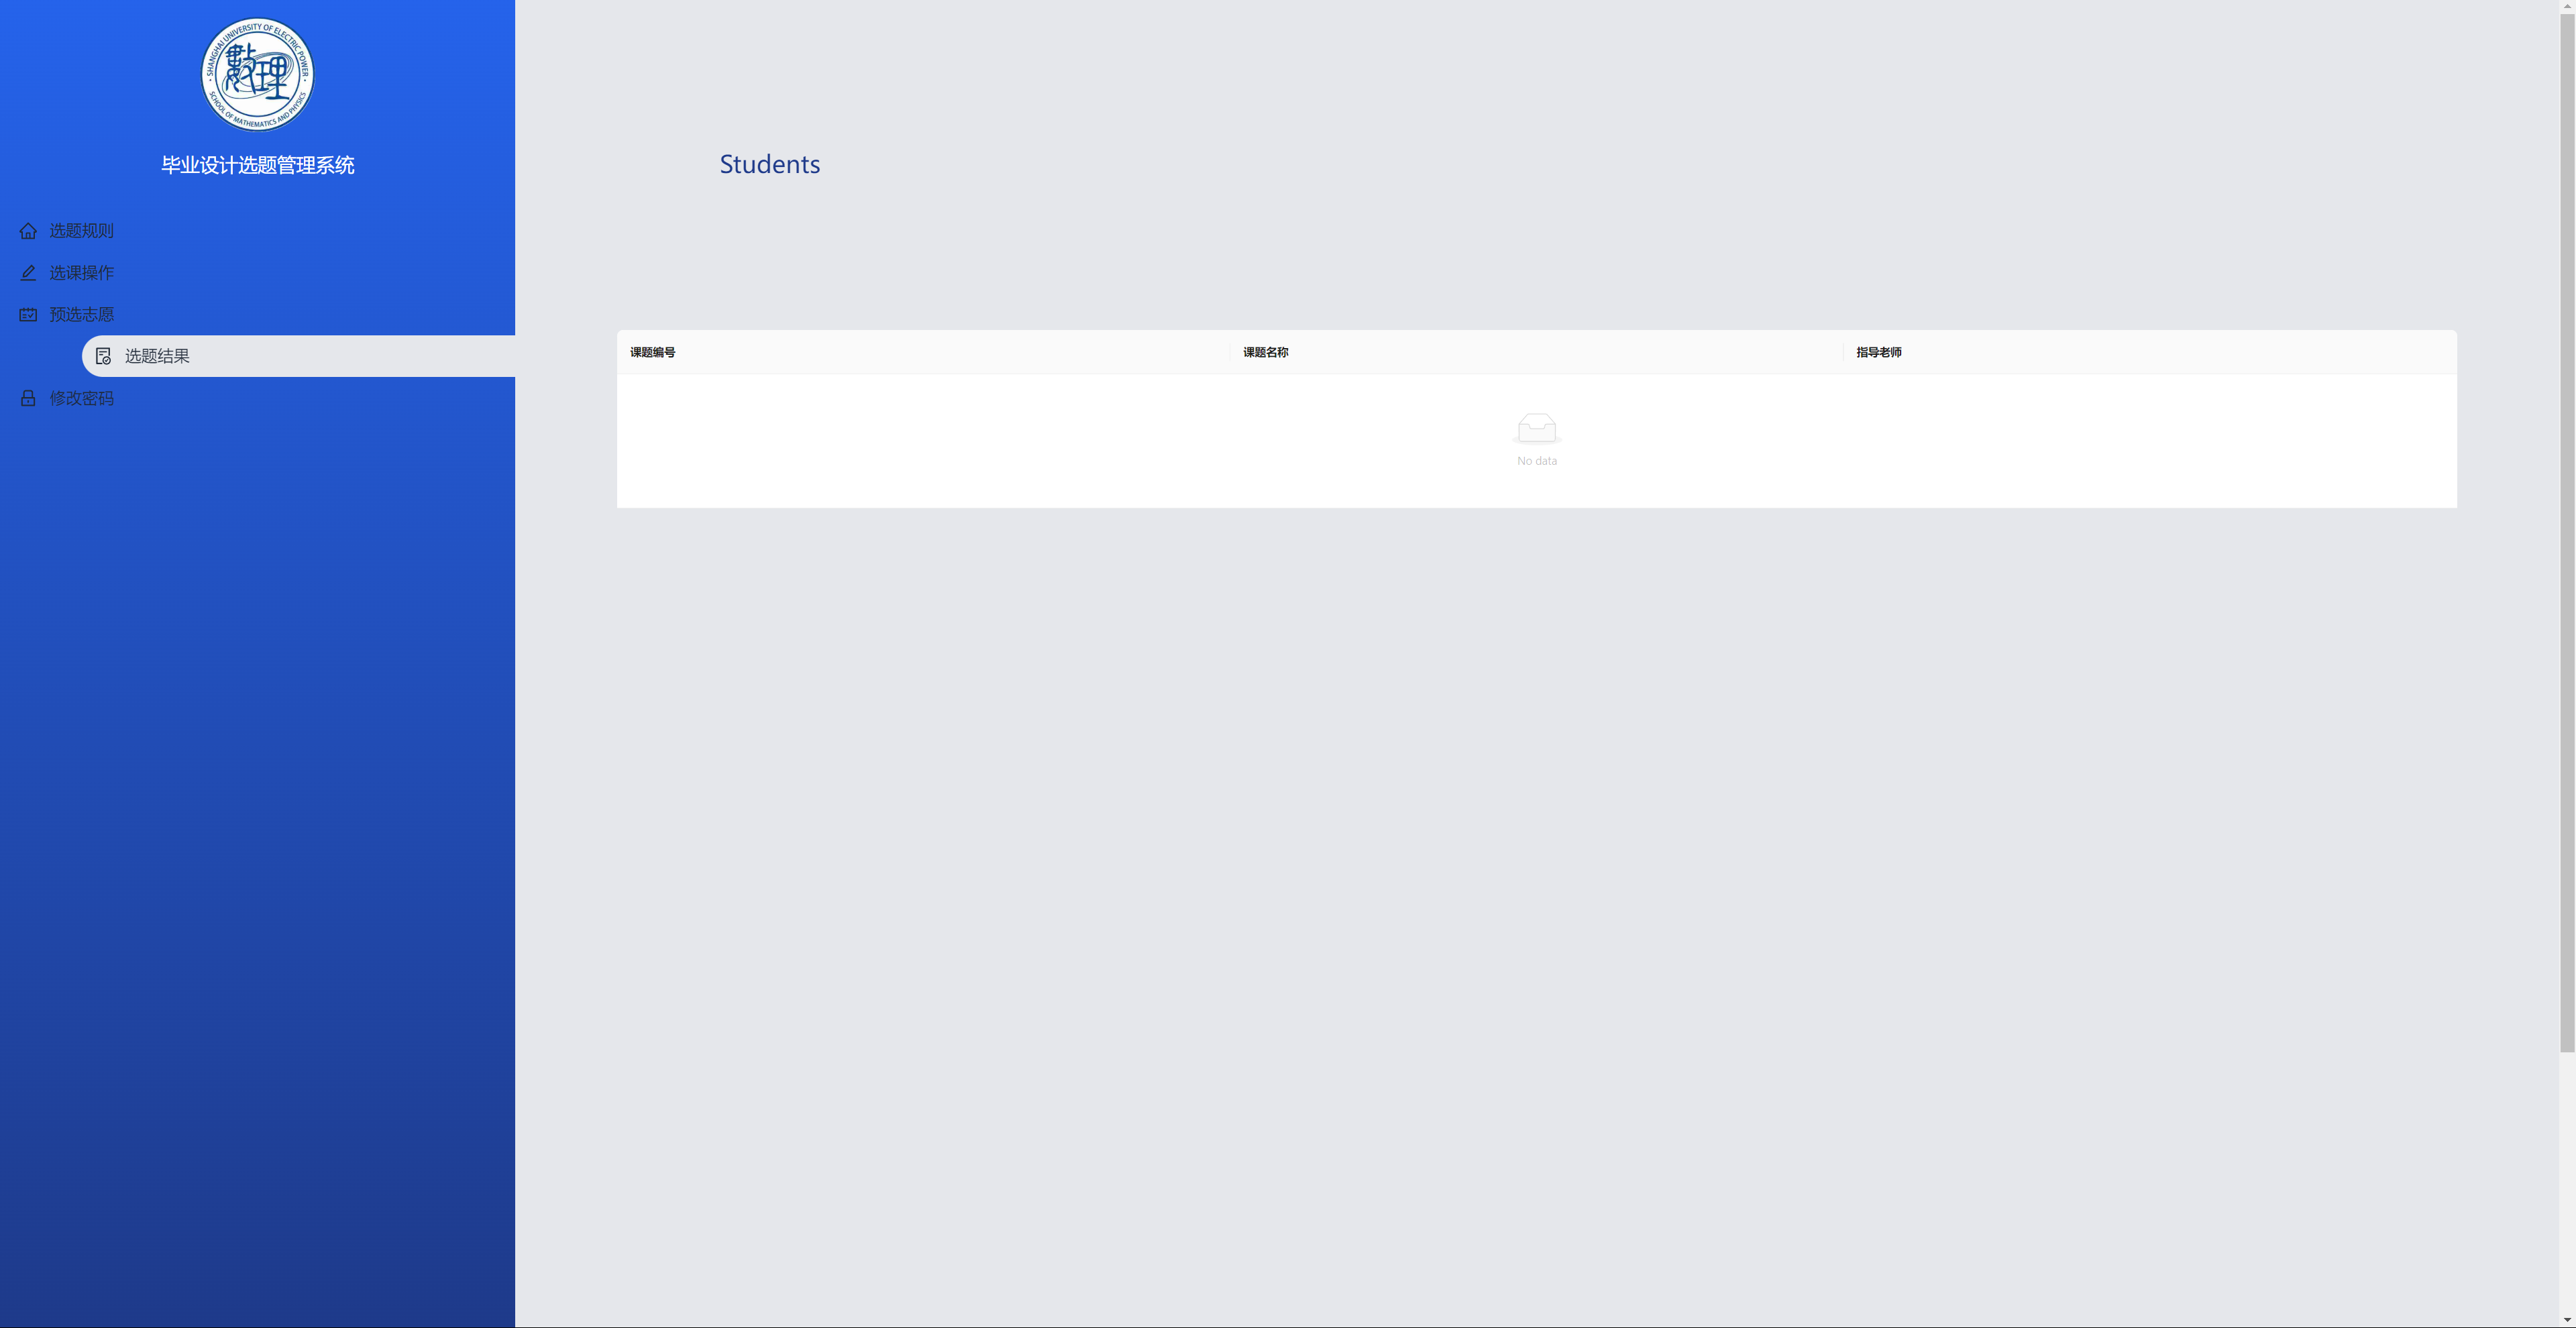
\includegraphics[width=1\textwidth]{学生端04.png}
    \caption{学生端-选题结果}
    \label{fig:student04}
\end{figure}

\clearpage

\subsubsection{修改密码:}
提供了学生更新密码的窗口。
\begin{figure}[ht]
    \centering
    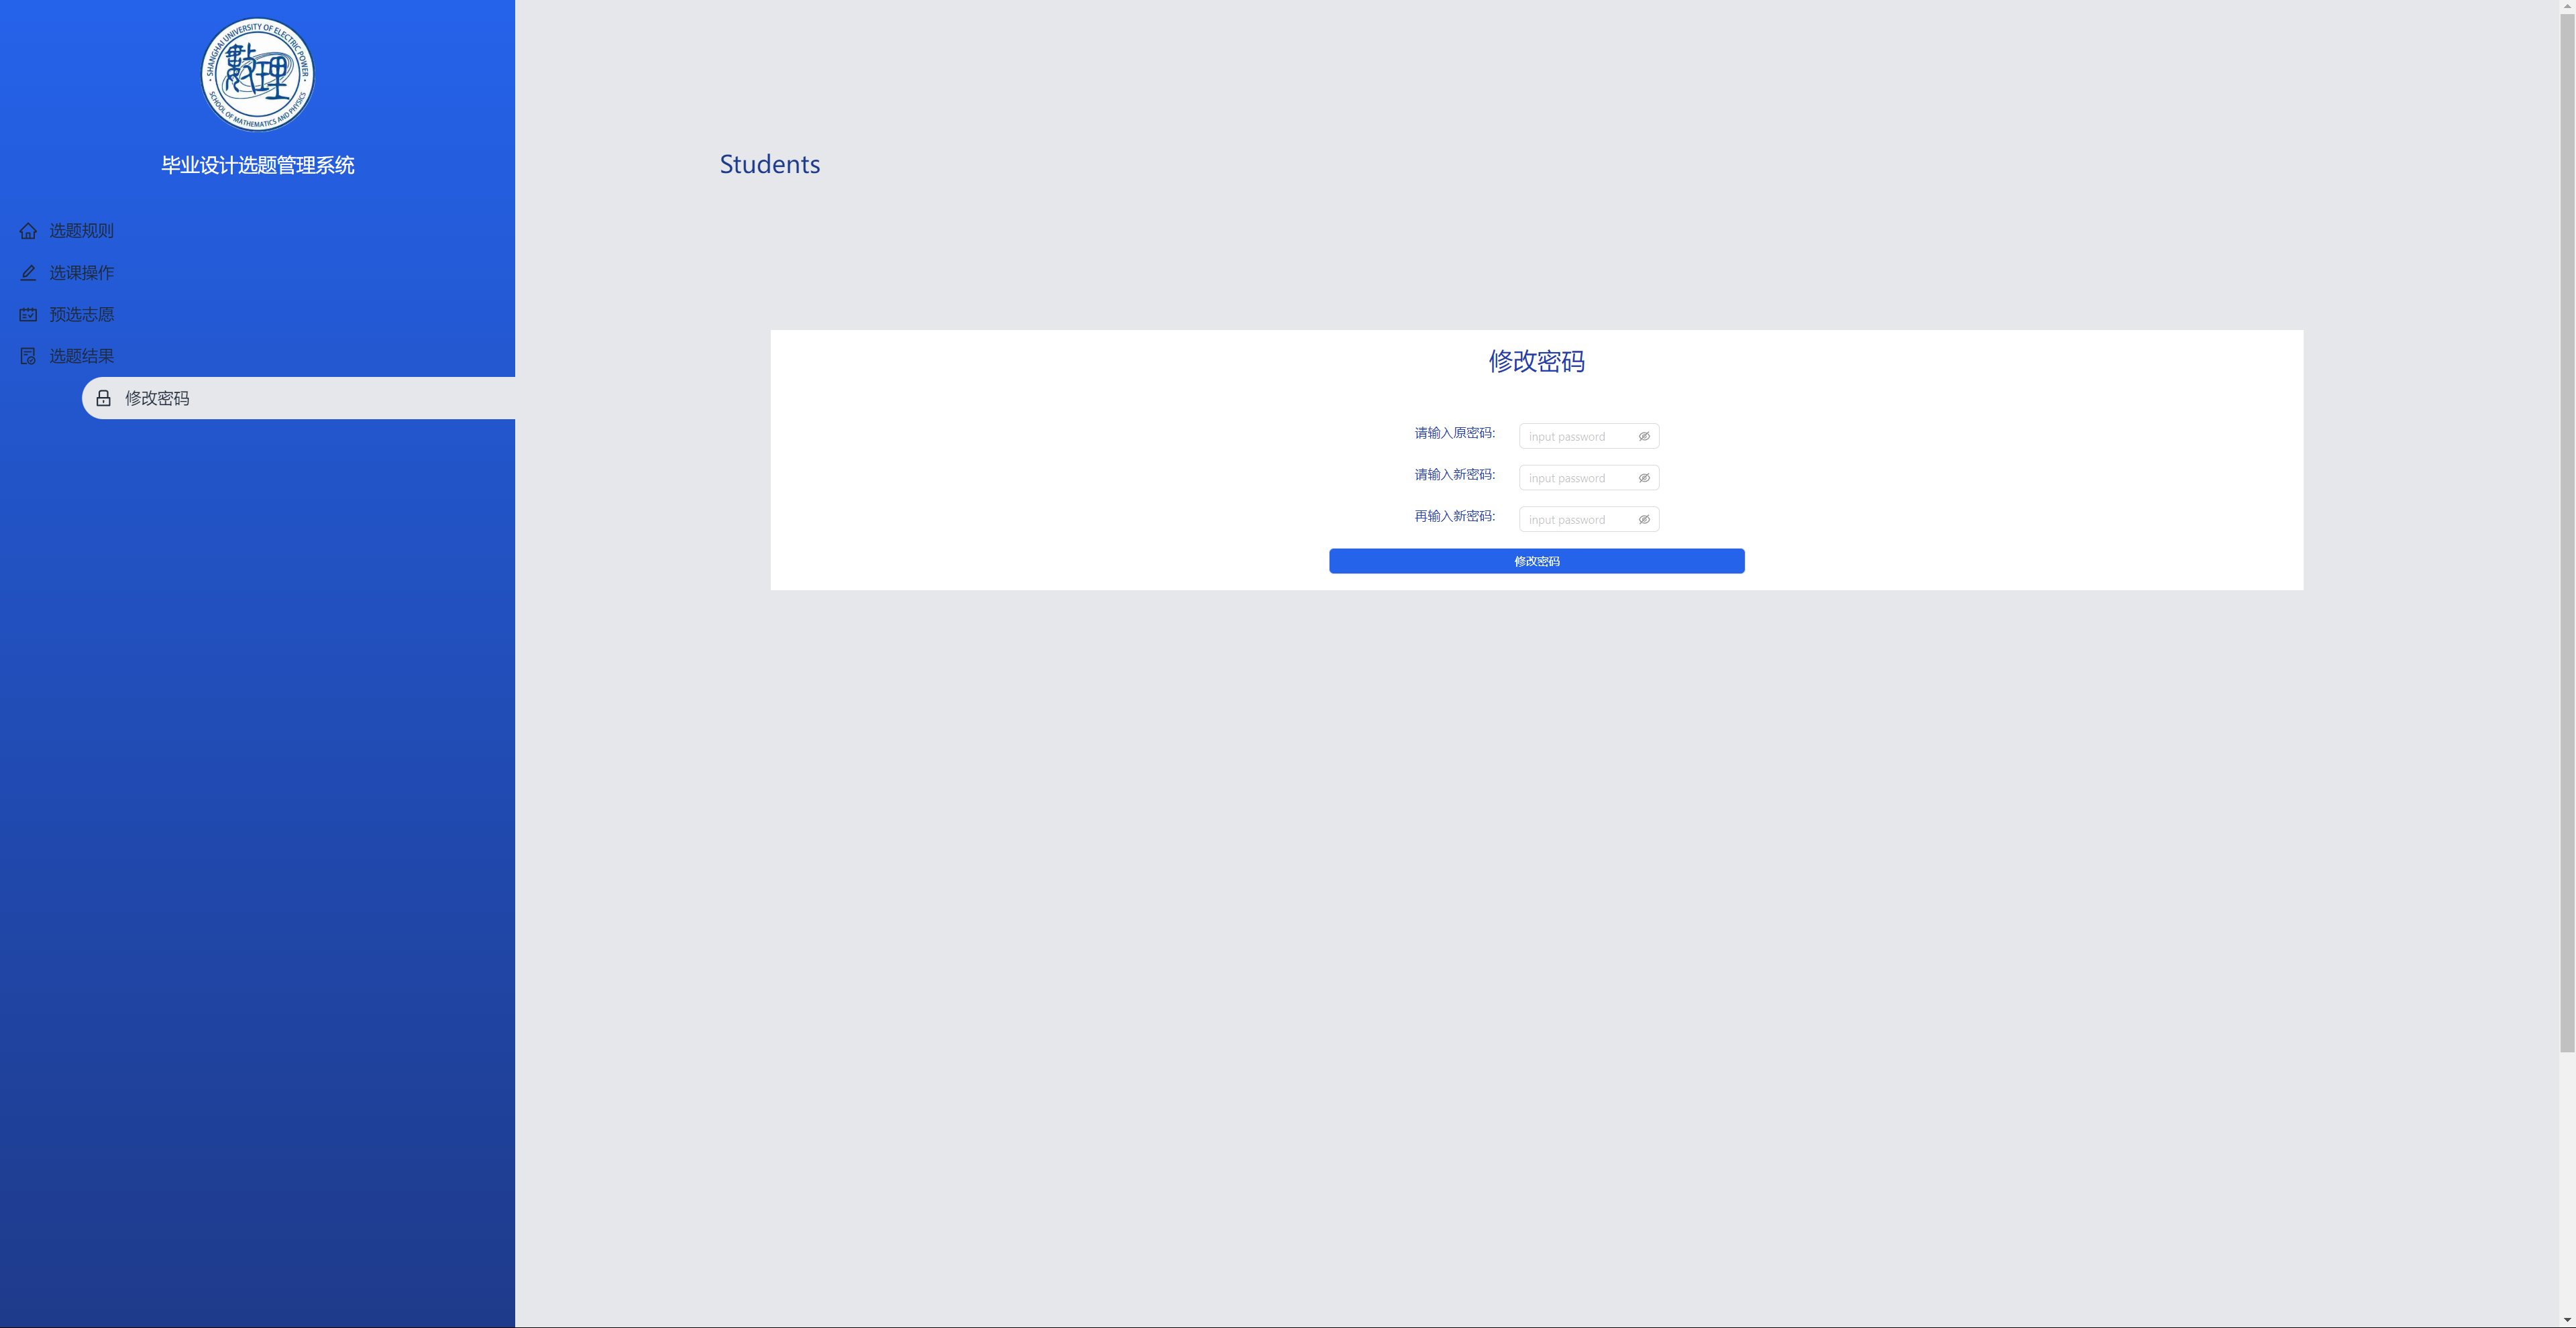
\includegraphics[width=1\textwidth]{学生端05.png}
    \caption{学生端-修改密码}
    \label{fig:student05}
\end{figure}